\documentclass[compress]{beamer}
\usepackage{ifthen,verbatim}

\newcommand{\isnote}{}
\xdefinecolor{lightyellow}{rgb}{1.,1.,0.25}
\xdefinecolor{darkblue}{rgb}{0.1,0.1,0.7}

%% Uncomment this to get annotations
%% \def\notes{\addtocounter{page}{-1}
%%            \renewcommand{\isnote}{*}
%% 	   \beamertemplateshadingbackground{lightyellow}{white}
%%            \begin{frame}
%%            \frametitle{Notes for the previous page (page \insertpagenumber)}
%%            \itemize}
%% \def\endnotes{\enditemize
%% 	      \end{frame}
%%               \beamertemplateshadingbackground{white}{white}
%%               \renewcommand{\isnote}{}}

%% Uncomment this to not get annotations
\def\notes{\comment}
\def\endnotes{\endcomment}

\setbeamertemplate{navigation symbols}{}
\setbeamertemplate{headline}{\mbox{ } \hfill
\begin{minipage}{5.5 cm}
\vspace{-0.75 cm} \small
\end{minipage} \hfill
\begin{minipage}{4.5 cm}
\vspace{-0.75 cm} \small
\begin{flushright}
\ifthenelse{\equal{\insertpagenumber}{1}}{}{Jim Pivarski \hspace{0.2 cm} \insertpagenumber\isnote/\pageref{numpages}}
\end{flushright}
\end{minipage}\mbox{\hspace{0.2 cm}}\includegraphics[height=1 cm]{../cmslogo} \hspace{0.1 cm} \includegraphics[height=1 cm]{../tamulogo} \hspace{0.01 cm} \vspace{-1.05 cm}}

\newcommand{\s}[1]{{\mbox{\scriptsize #1}}}

\begin{document}
%% \begin{notes}
%% \item This is the annotated version of my talk.
%% \item If you want the version that I am presenting, download the one
%% labeled ``slides'' on Indico (or just ignore these yellow pages).
%% \item The annotated version is provided for extra detail and a written
%% record of comments that I intend to make orally.
%% \item Yellow notes refer to the content on the {\it previous} page.
%% \item All other slides are identical for the two versions.
%% \end{notes}

\small

%% \begin{frame}
%% \frametitle{Outline}
%% \begin{itemize}\setlength{\itemsep}{0.75 cm}
%% \item 
%% \end{itemize}
%% %% \hspace{-0.83 cm} \textcolor{darkblue}{\Large Outline2}
%% \end{frame}

\begin{frame}
\frametitle{Drell-Yan normalization}

\begin{columns}
\column{0.5\linewidth}
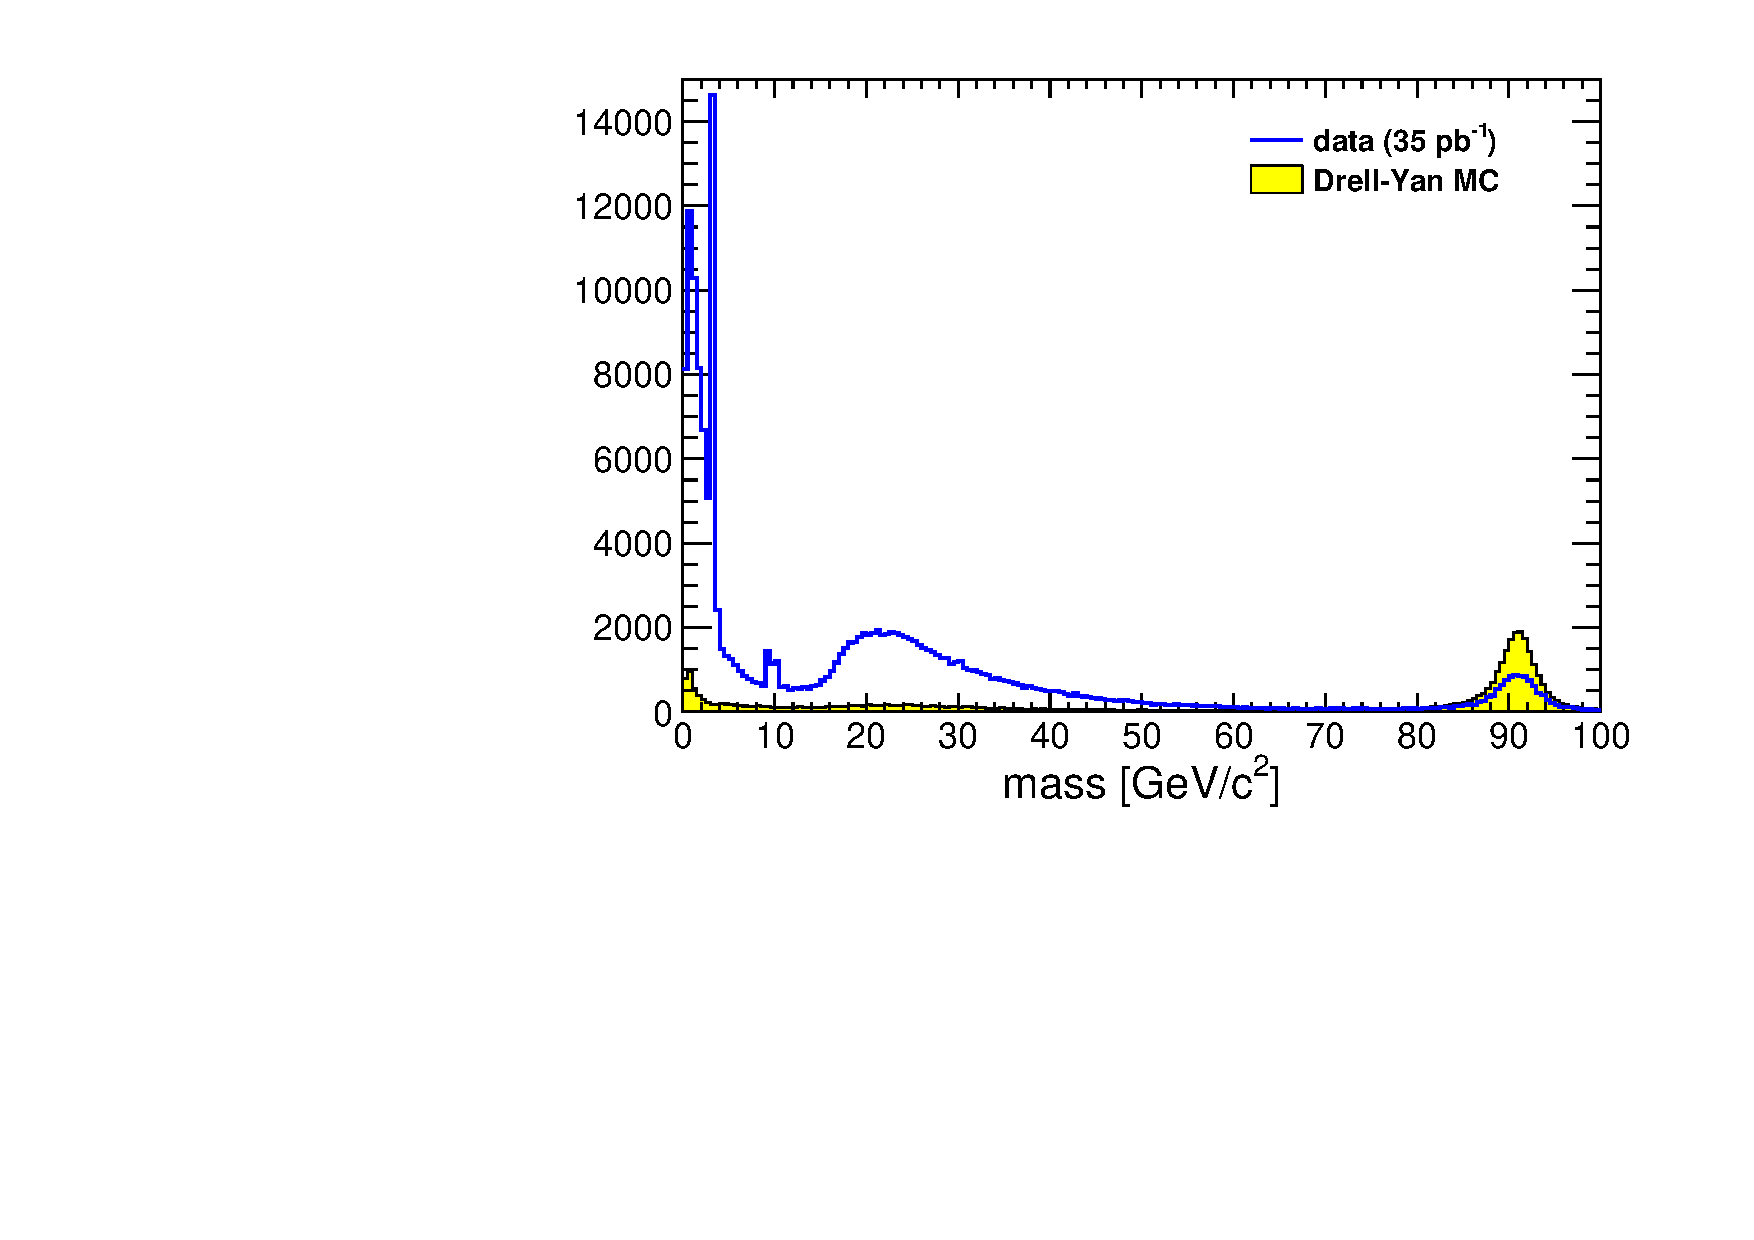
\includegraphics[width=\linewidth]{normalizing_to_the_z_naive.pdf}

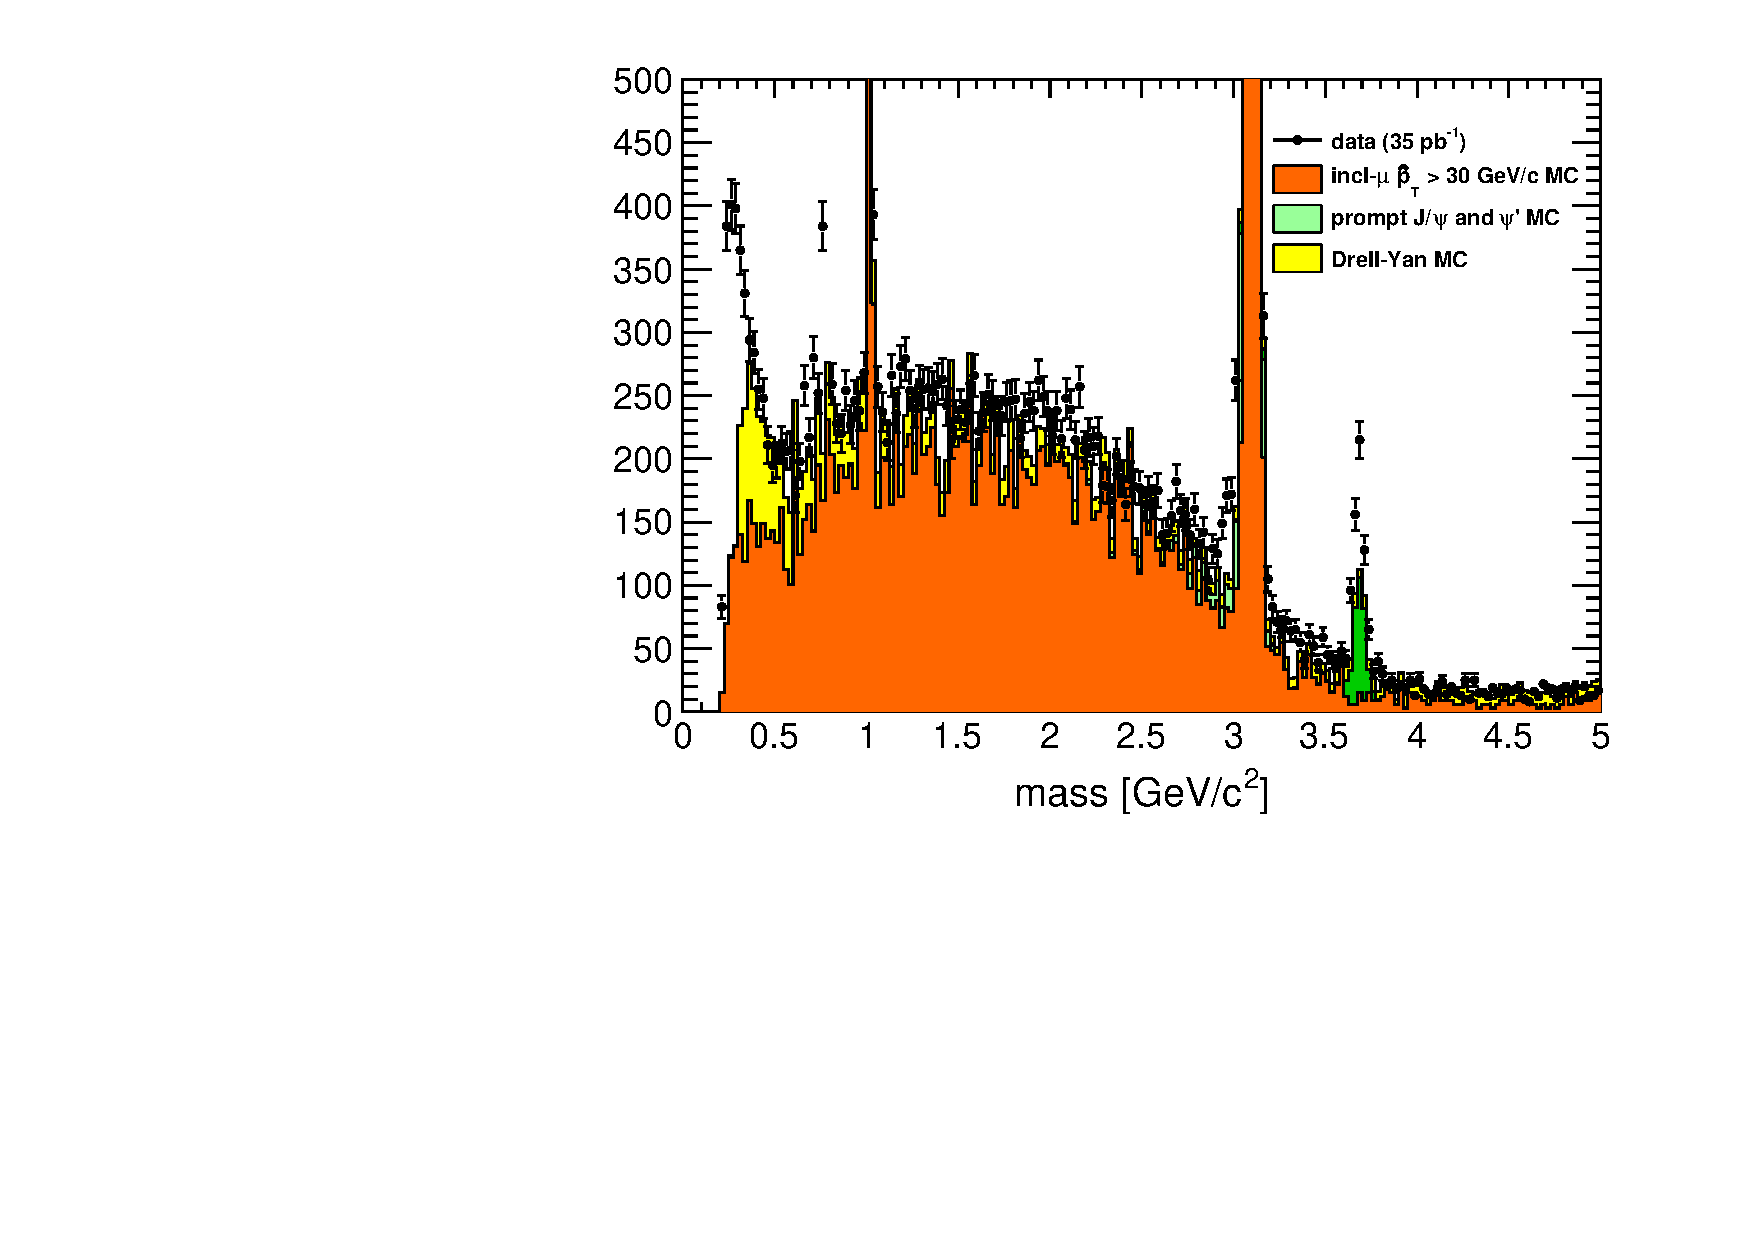
\includegraphics[width=\linewidth]{lowdimuon_mass_nobcuts_naive.pdf}

\column{0.5\linewidth}
\begin{itemize}
\item After fixing a few misinterpretations of the Pythia
  cross-section output, it seems to be about right for the low-mass
  region and a factor of two too high for the $Z$
\end{itemize}
\end{columns}
\end{frame}

\begin{frame}
\frametitle{Drell-Yan normalization}

\begin{columns}
\column{0.5\linewidth}
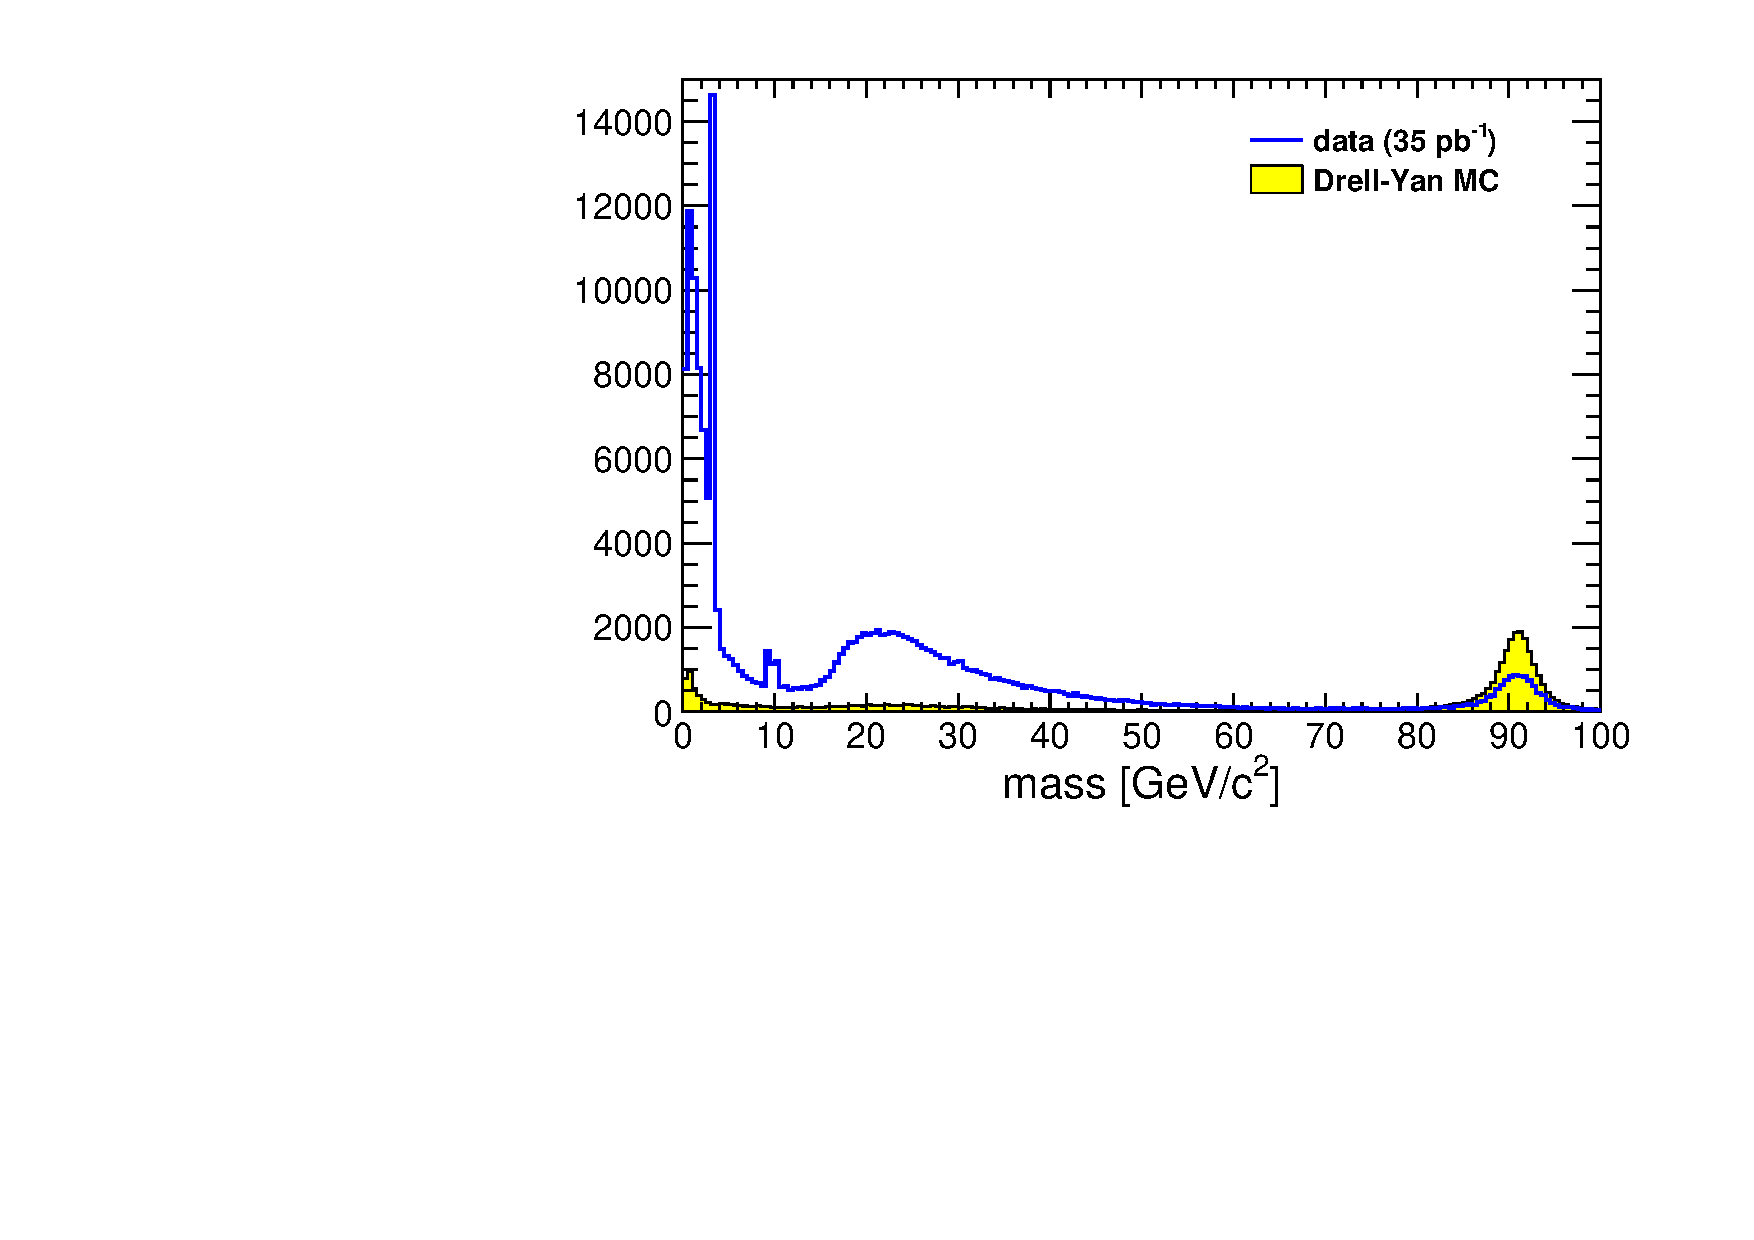
\includegraphics[width=\linewidth]{normalizing_to_the_z_naive.pdf}

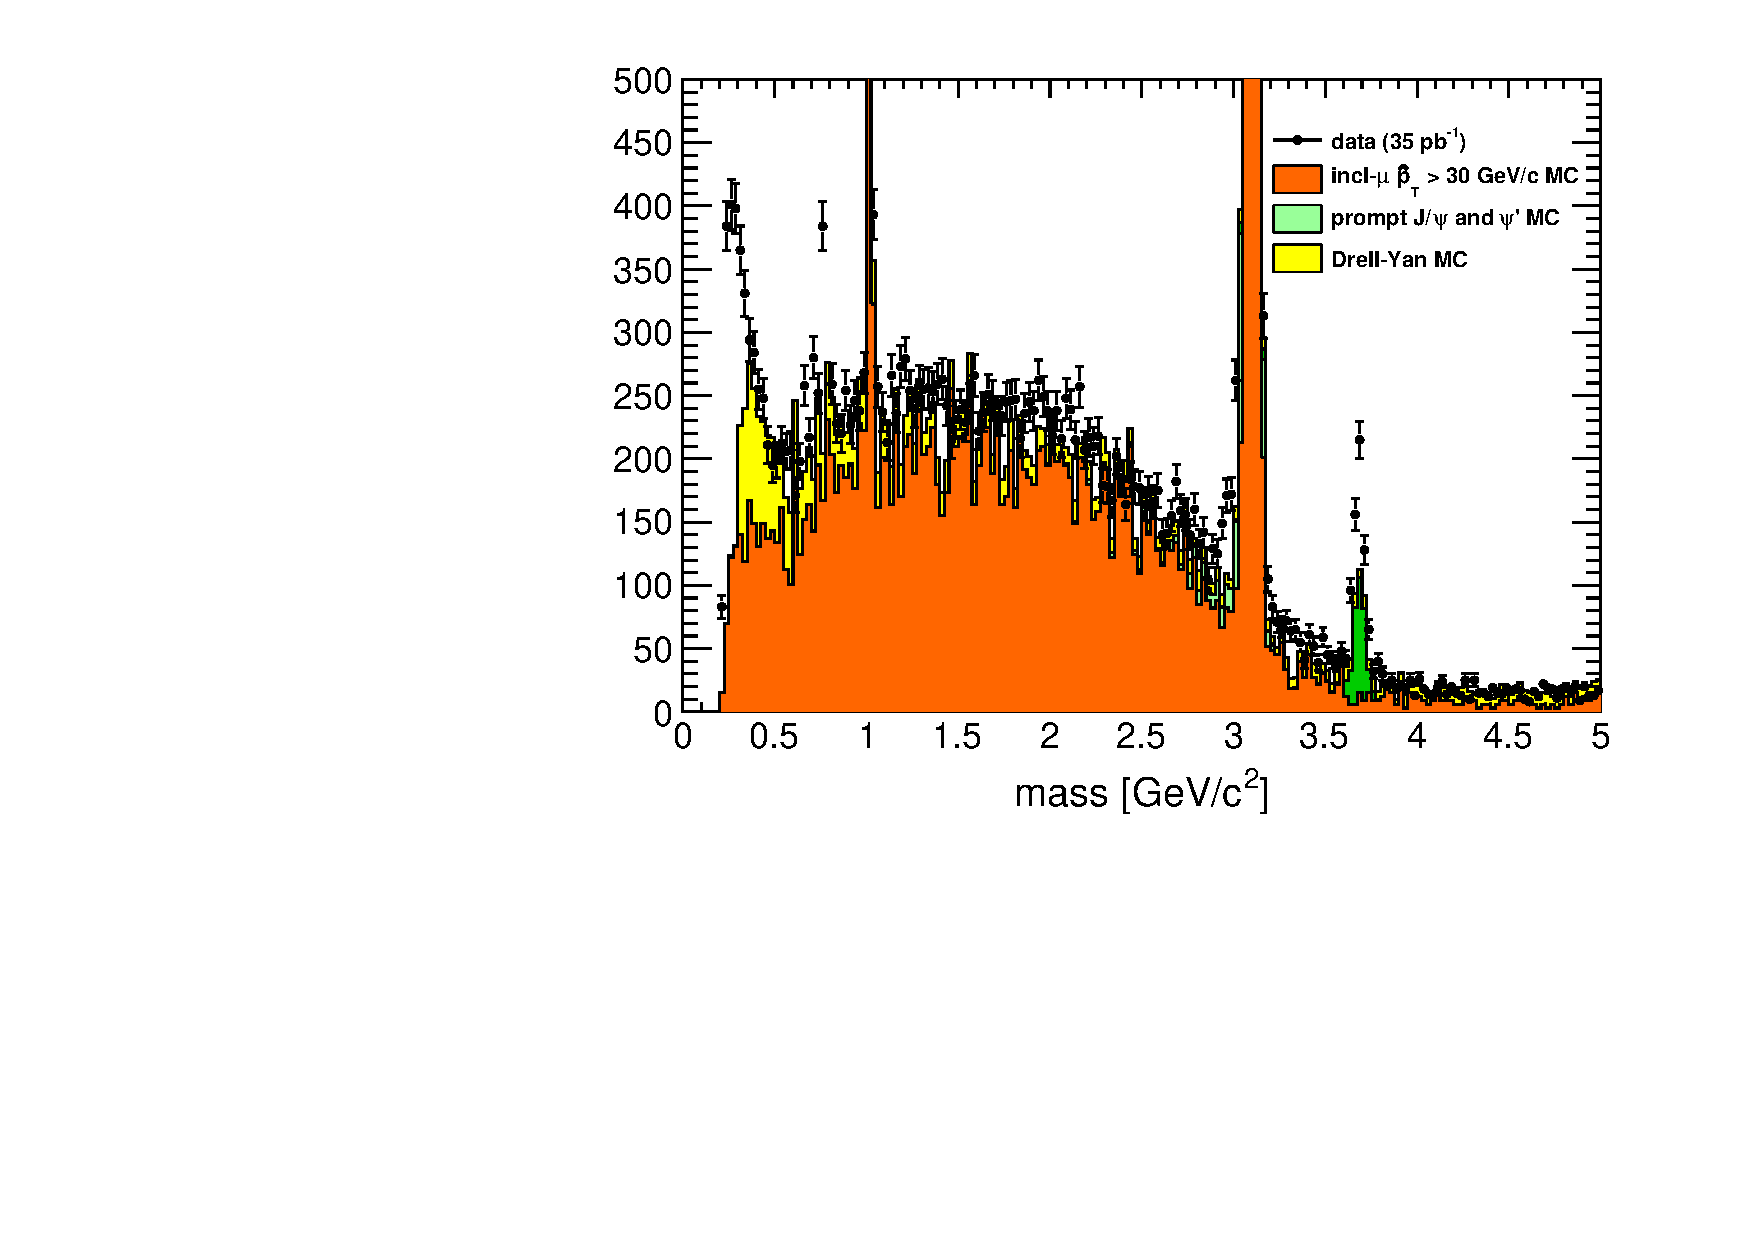
\includegraphics[width=\linewidth]{lowdimuon_mass_nobcuts_naive.pdf}

\column{0.5\linewidth}
\begin{itemize}
\item Changing the generator-level mass cut doesn't give me a factor of two (below)
\item The usual mode of operation would be to only run this for masses
  above 40~GeV/$c^2$
\end{itemize}

\mbox{\hspace{-0.75 cm}\begin{tabular}{c c c c}
\scriptsize min $\hat{p}_T$ & \scriptsize min $m$ & \scriptsize max $m$ & \scriptsize intlumi (mb$^{-1}$) \\\hline
\scriptsize   10.  &  \scriptsize 0.05 & \scriptsize $\infty$ & \scriptsize   10000/2.912$\times 10^{-5}$ \\
\scriptsize   10.  &  \scriptsize 0.05 & \scriptsize  5     &  \scriptsize  10000/1.137$\times 10^{-5}$ \\
\scriptsize   10.  &  \scriptsize 40  & \scriptsize $\infty$ & \scriptsize   10000/1.166$\times 10^{-6}$ \\
\end{tabular}}

\vspace{0.5 cm}
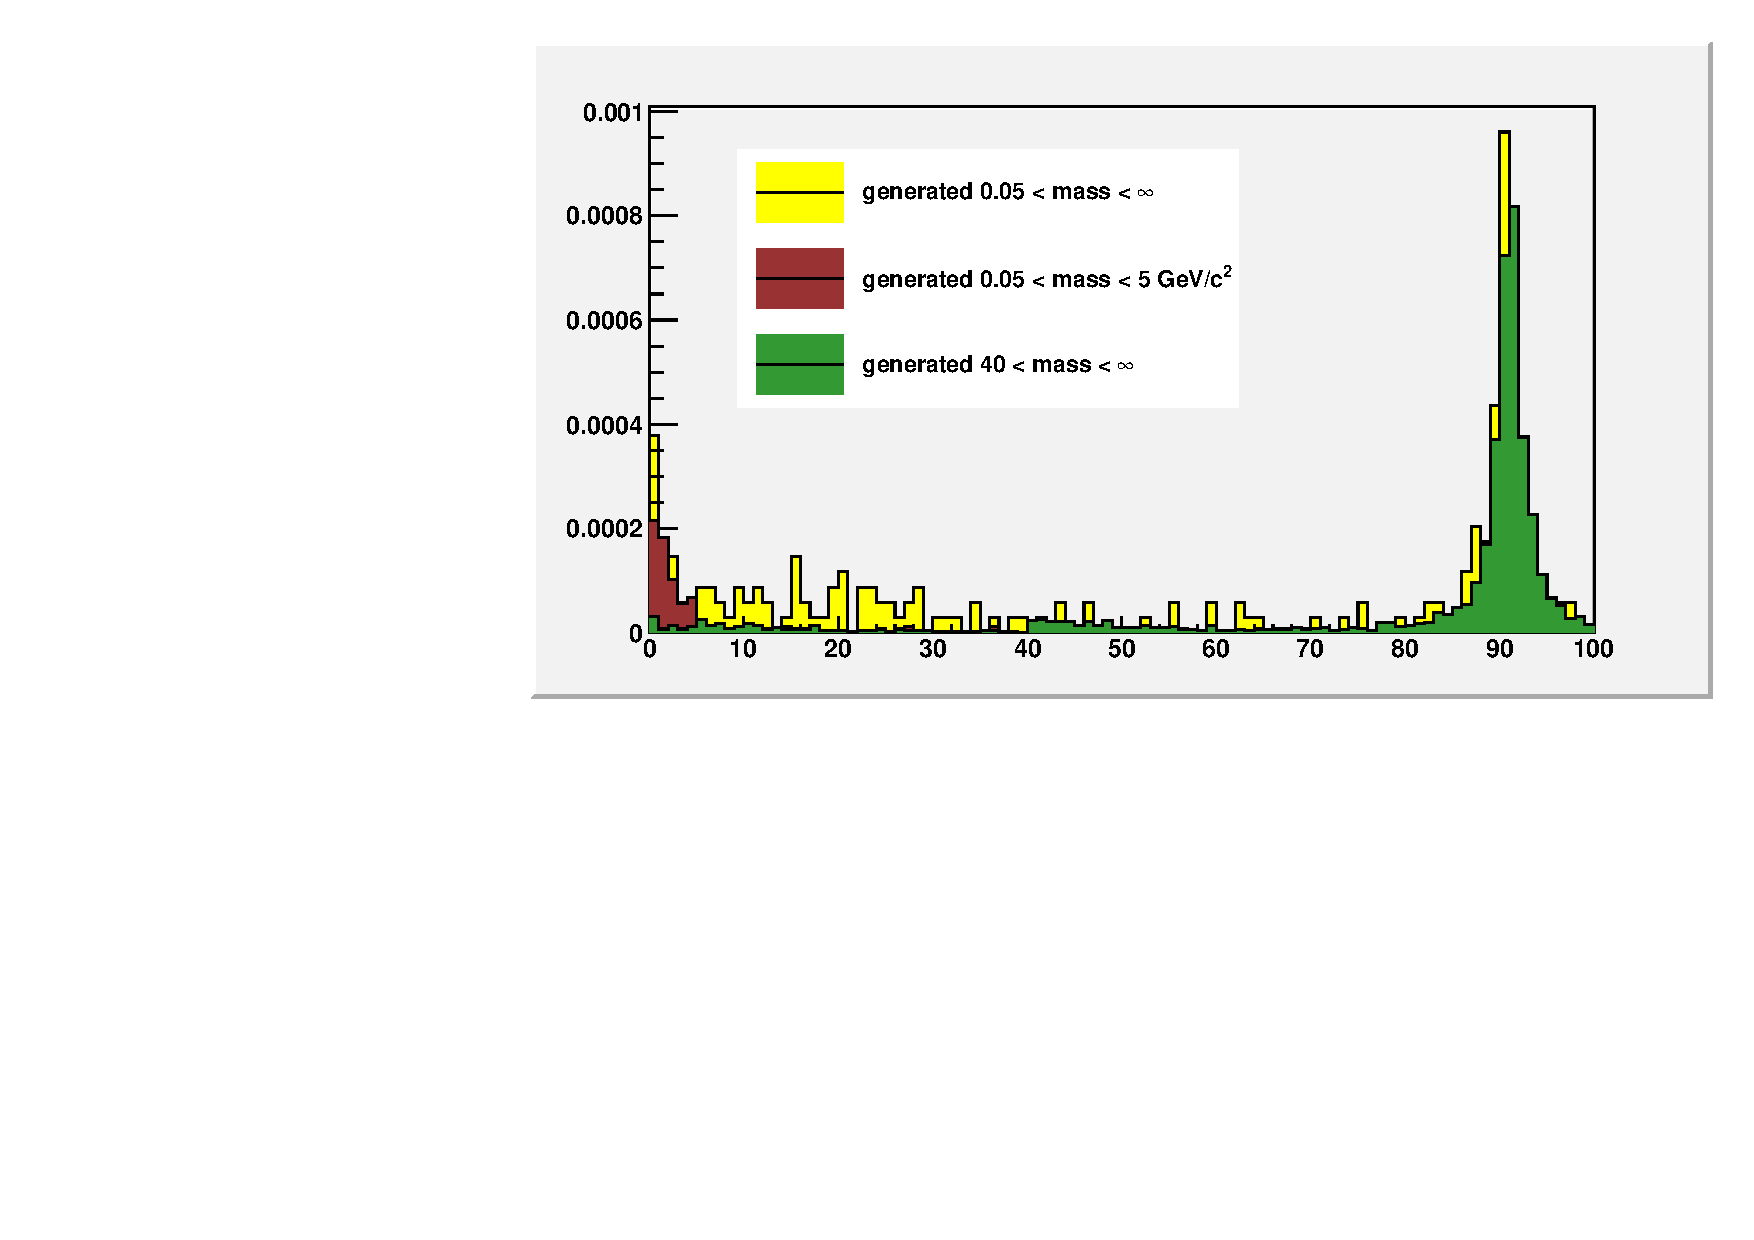
\includegraphics[width=\linewidth]{crosssec_mcuts.pdf}
\end{columns}
\end{frame}

\begin{frame}
\frametitle{Drell-Yan normalization}

\begin{columns}
\column{0.5\linewidth}
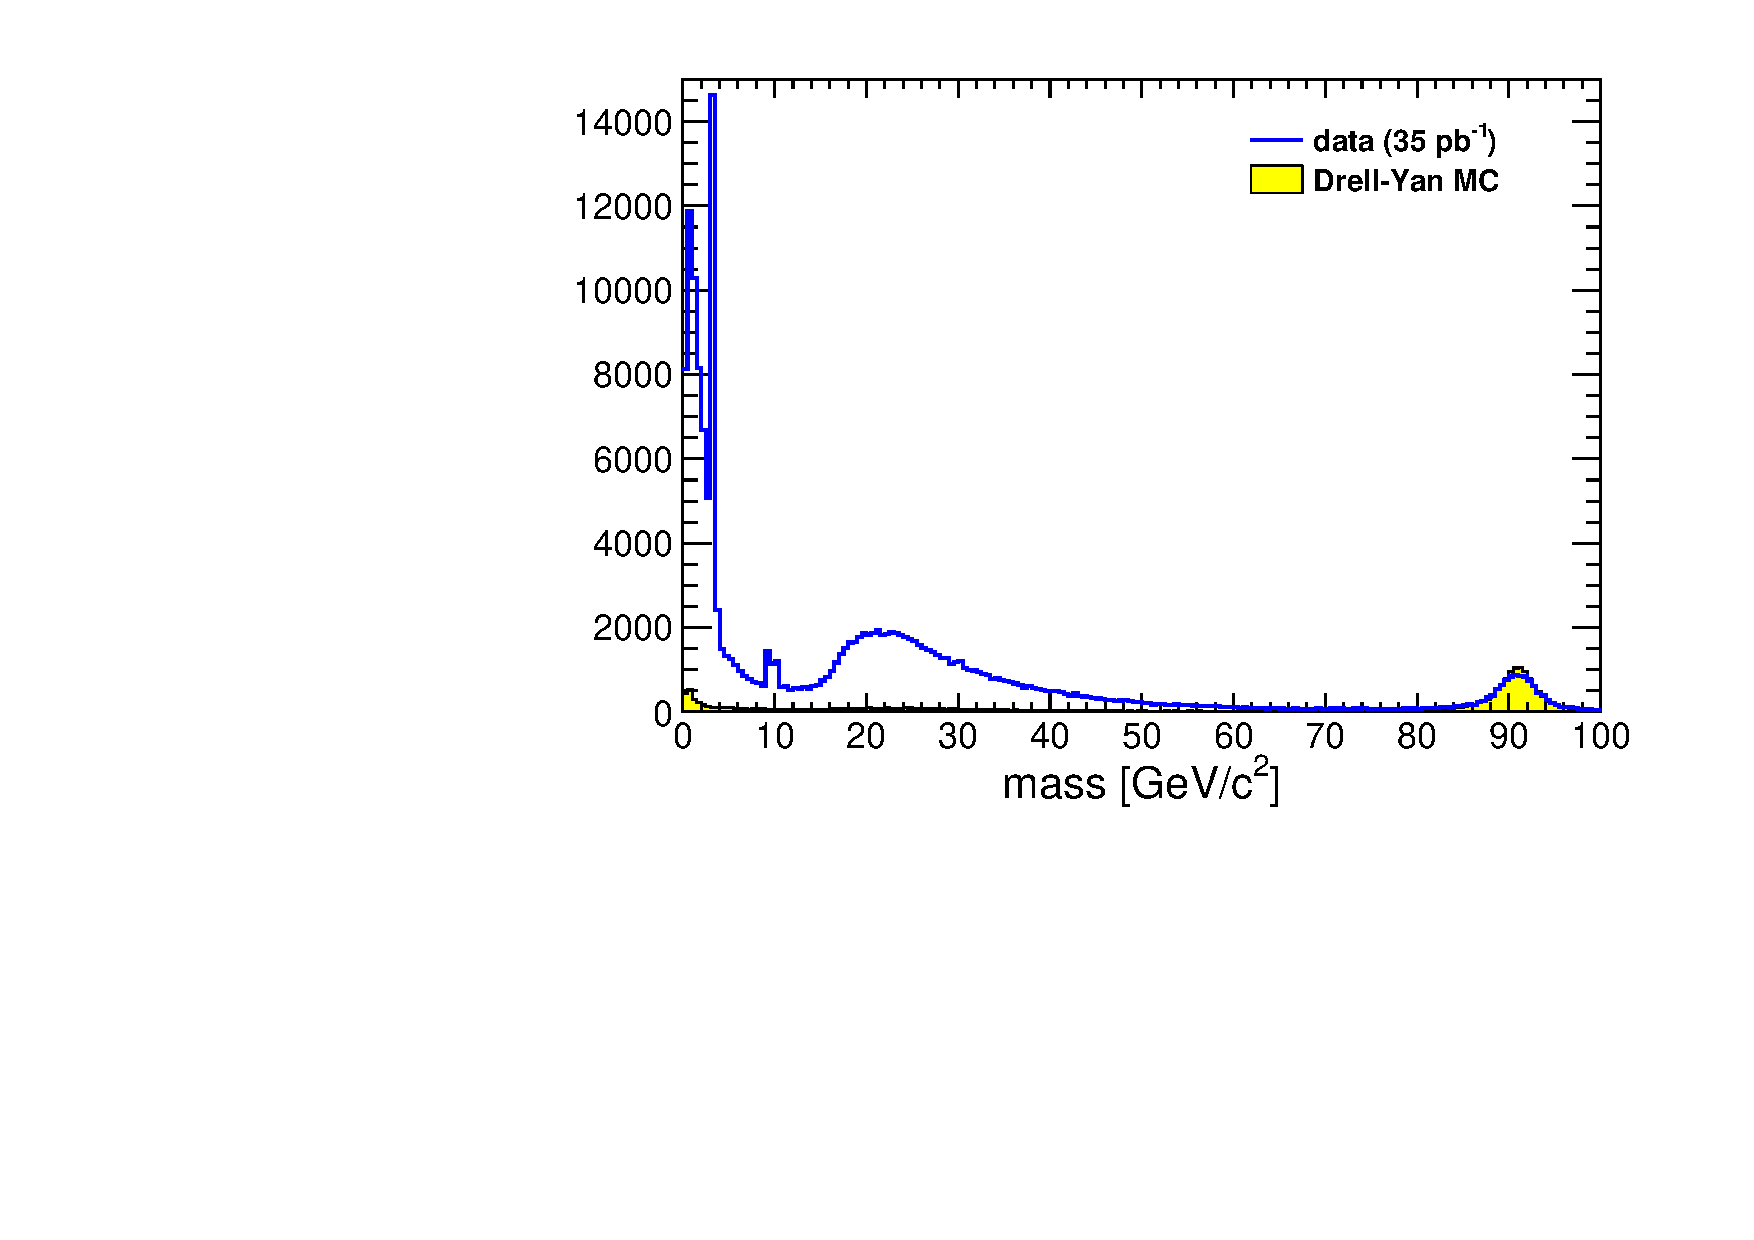
\includegraphics[width=\linewidth]{normalizing_to_the_z.pdf}

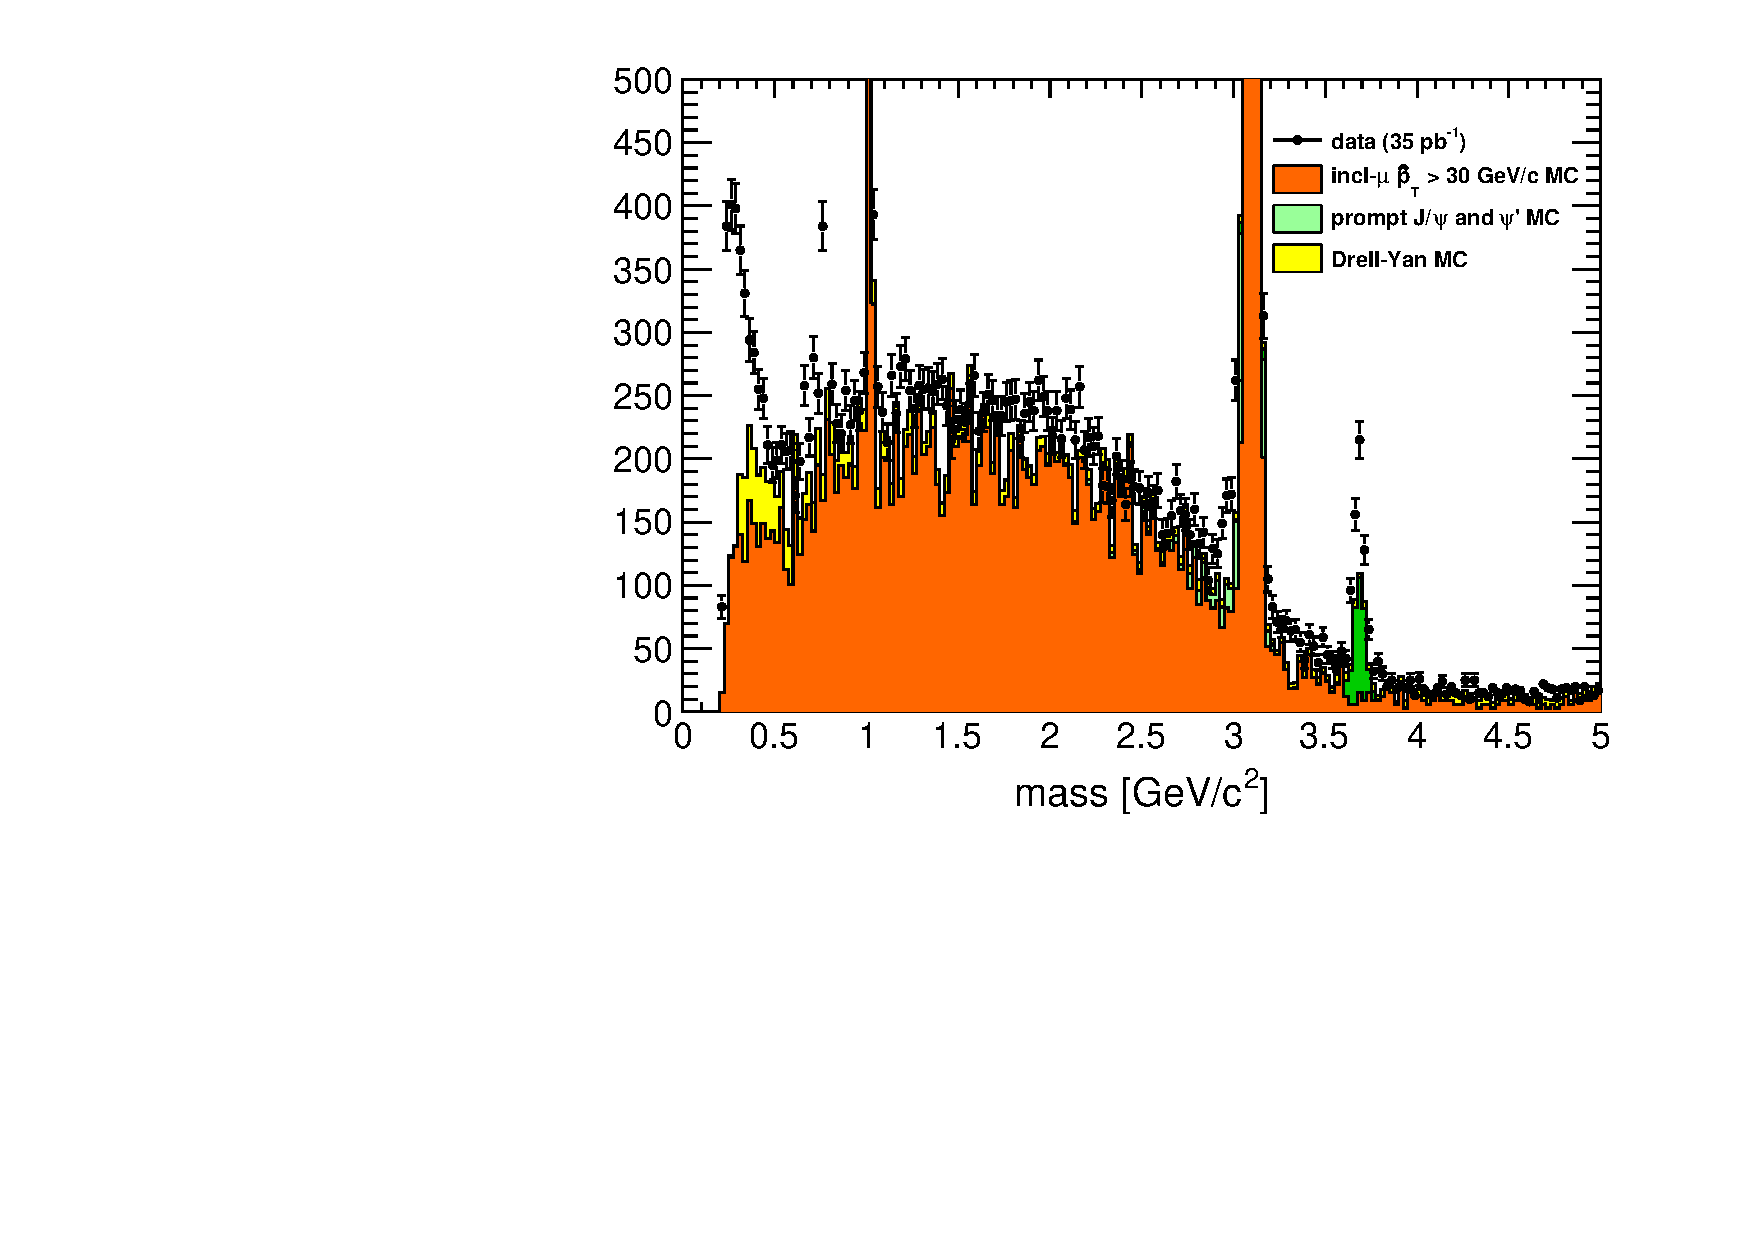
\includegraphics[width=\linewidth]{lowdimuon_mass_nobcuts.pdf}

\column{0.5\linewidth}
\begin{itemize}
\item Explicitly scaling to the $Z$ (left) yields an equally
  believable spectrum: we don't know how much of the data-excess is
  actually more $b\bar{b}$, rather than Drell-Yan
\item I'll use this scaling for the rest of the talk and minimize
  dependence on the Drell-Yan MC
\item We can, for instance, be guided by the MC's isolation and
  $L_{xy}$ (flight distance), since that is mostly detector simulation
\end{itemize}

\end{columns}
\end{frame}

\begin{frame}
\frametitle{$b\bar{b}$ cuts for mass template}

\begin{itemize}
\item Only $b\bar{b} \to 2\mu X, \, 2\mu X$ can appear in the
  dimuon-dimuon sample, so our mass template must be constructed from
  $b \to 2\mu X$
\end{itemize}

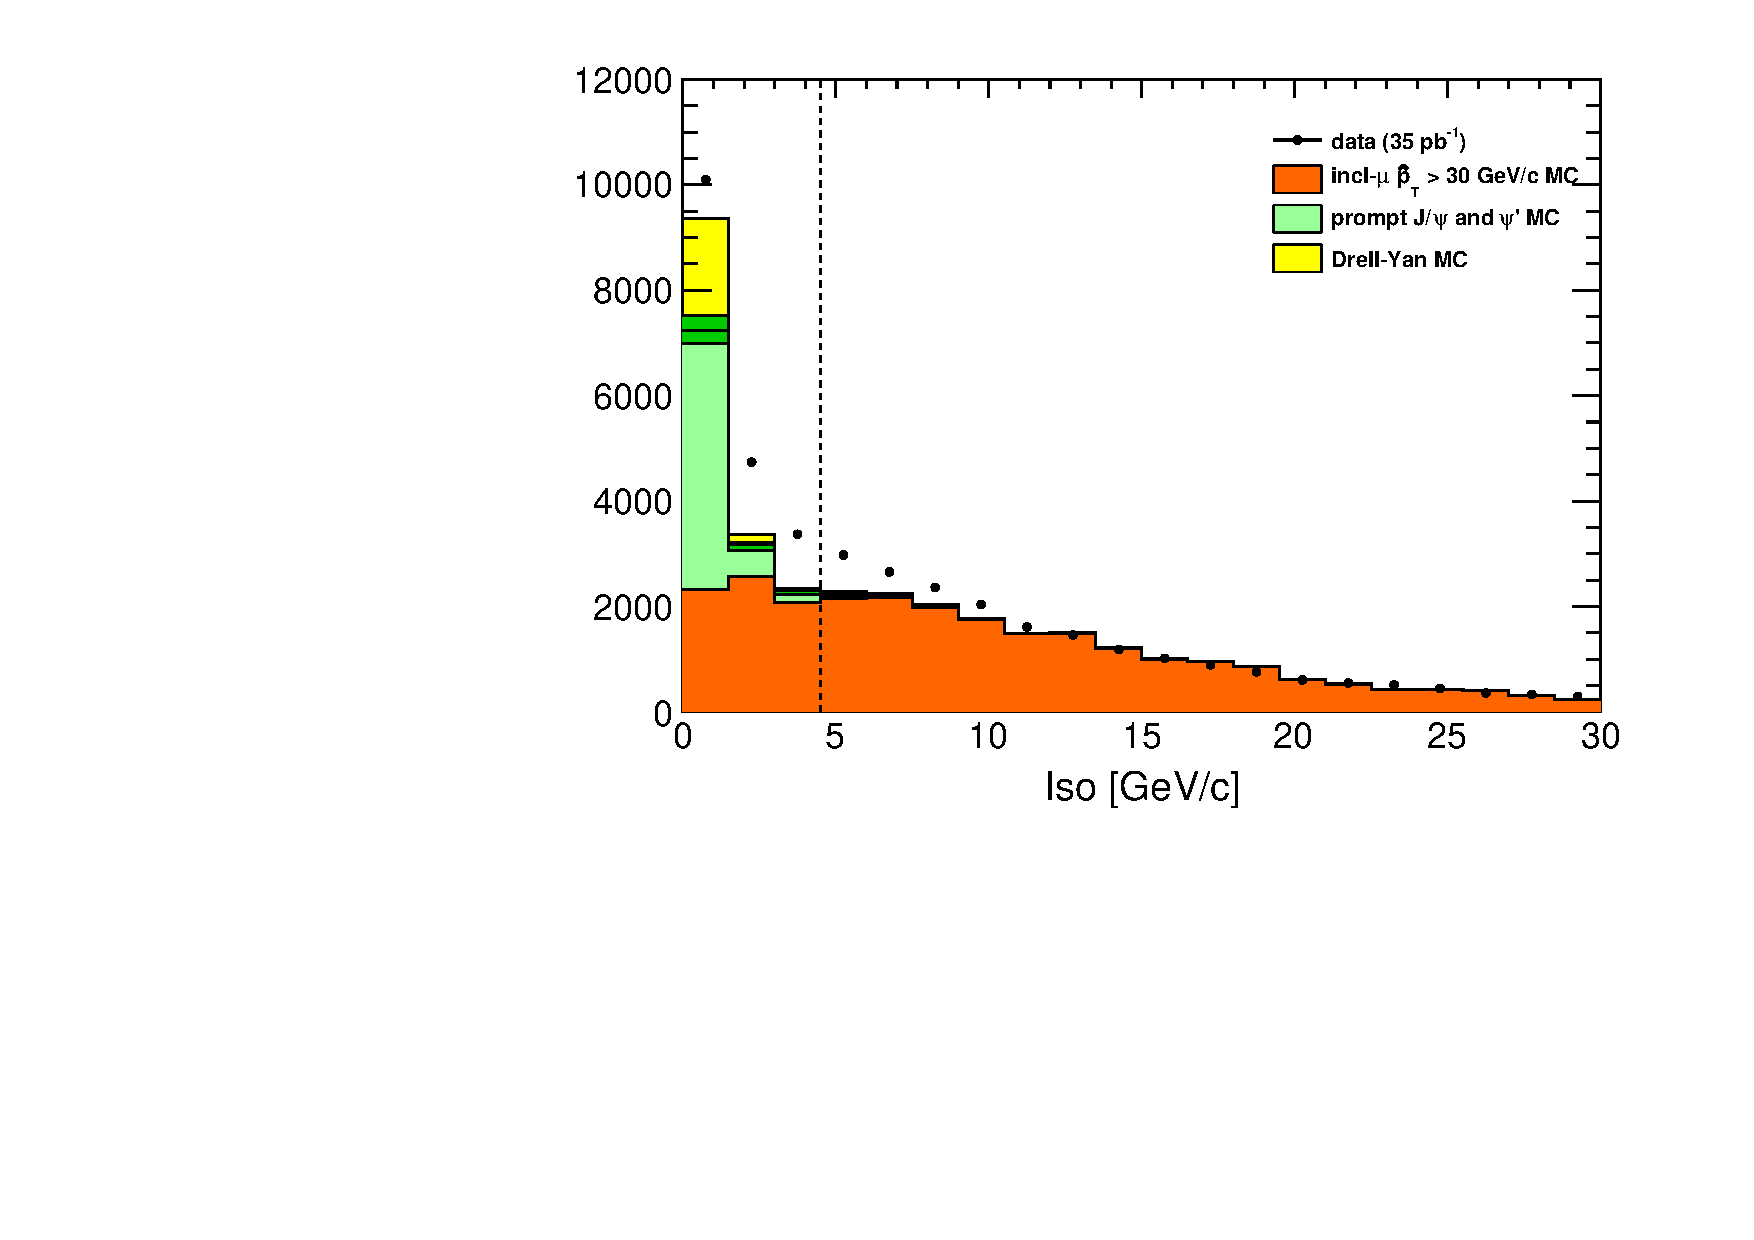
\includegraphics[width=0.5\linewidth]{lowdimuon_iso_everything.pdf}
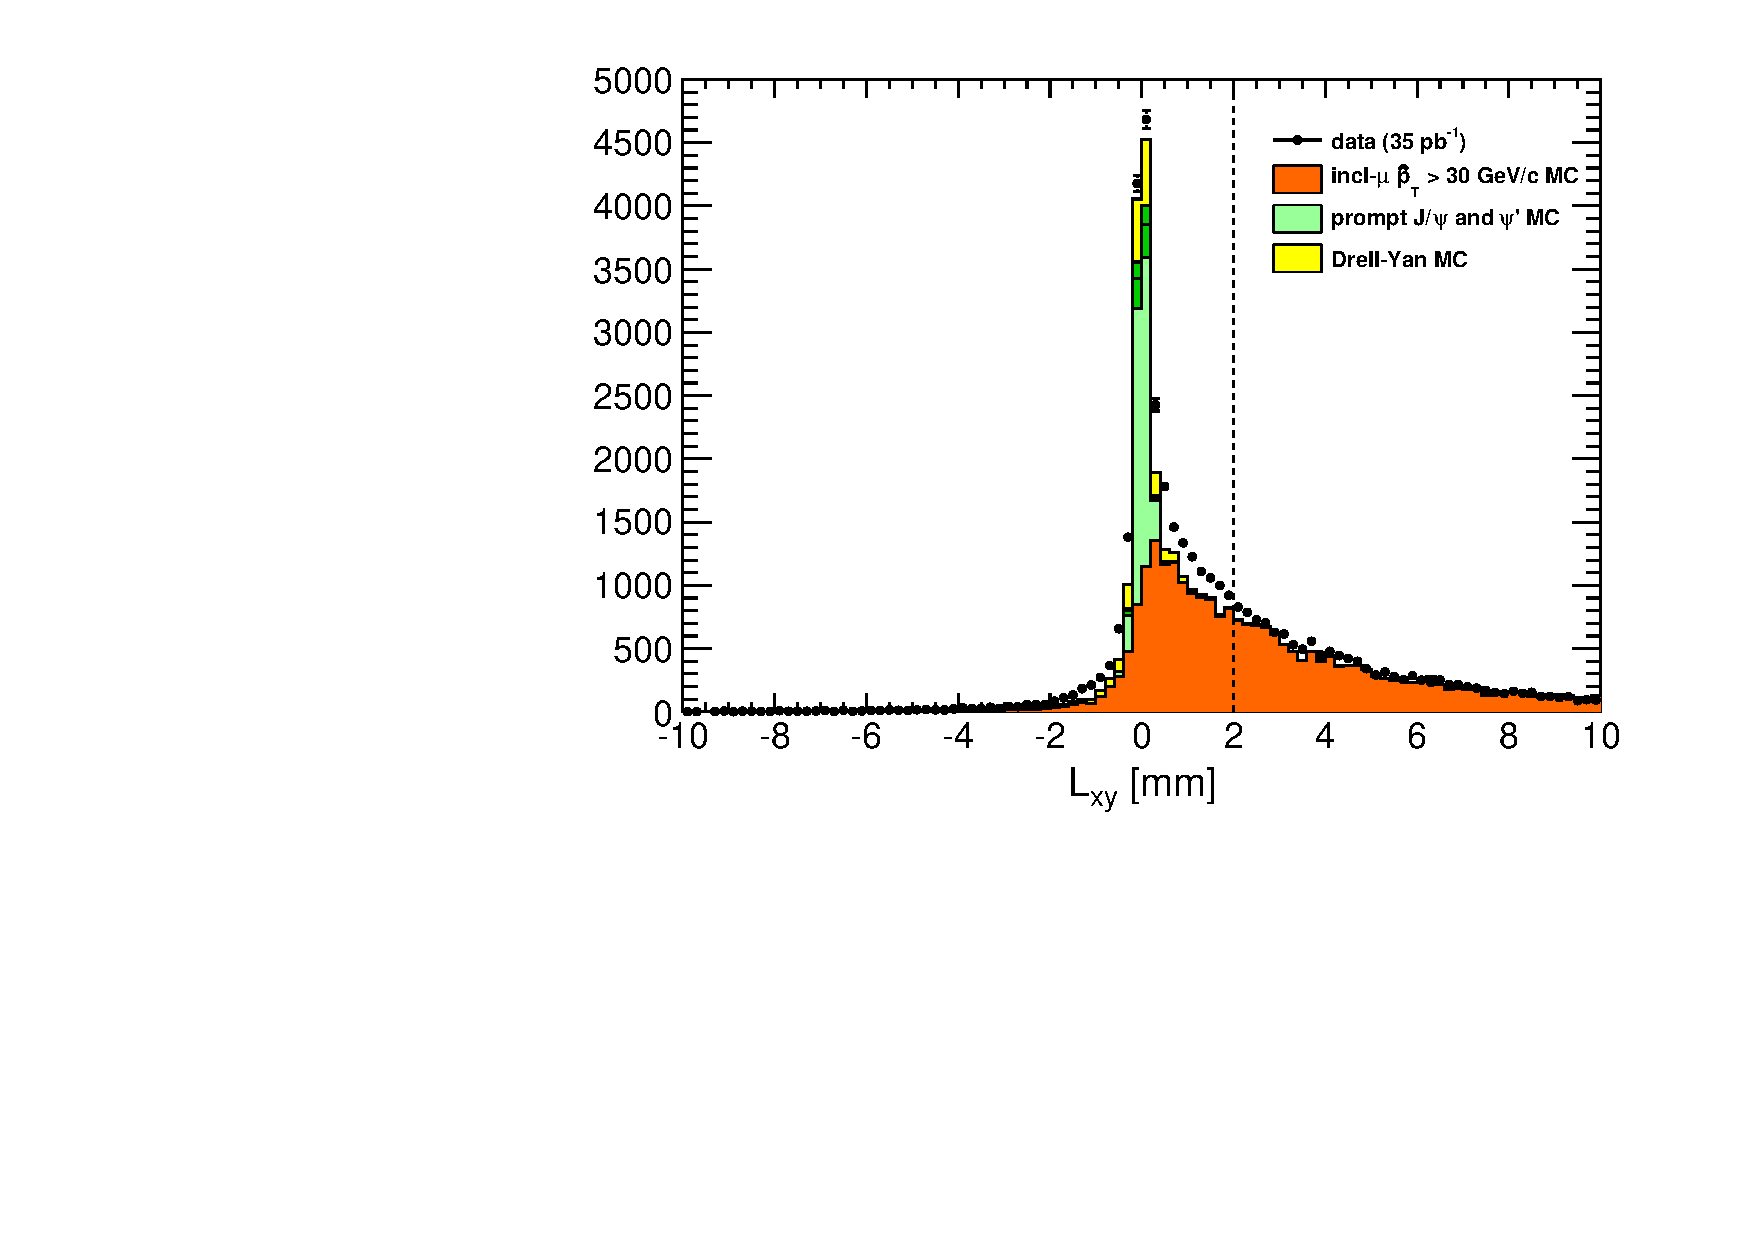
\includegraphics[width=0.5\linewidth]{lowdimuon_lxy_everything.pdf}

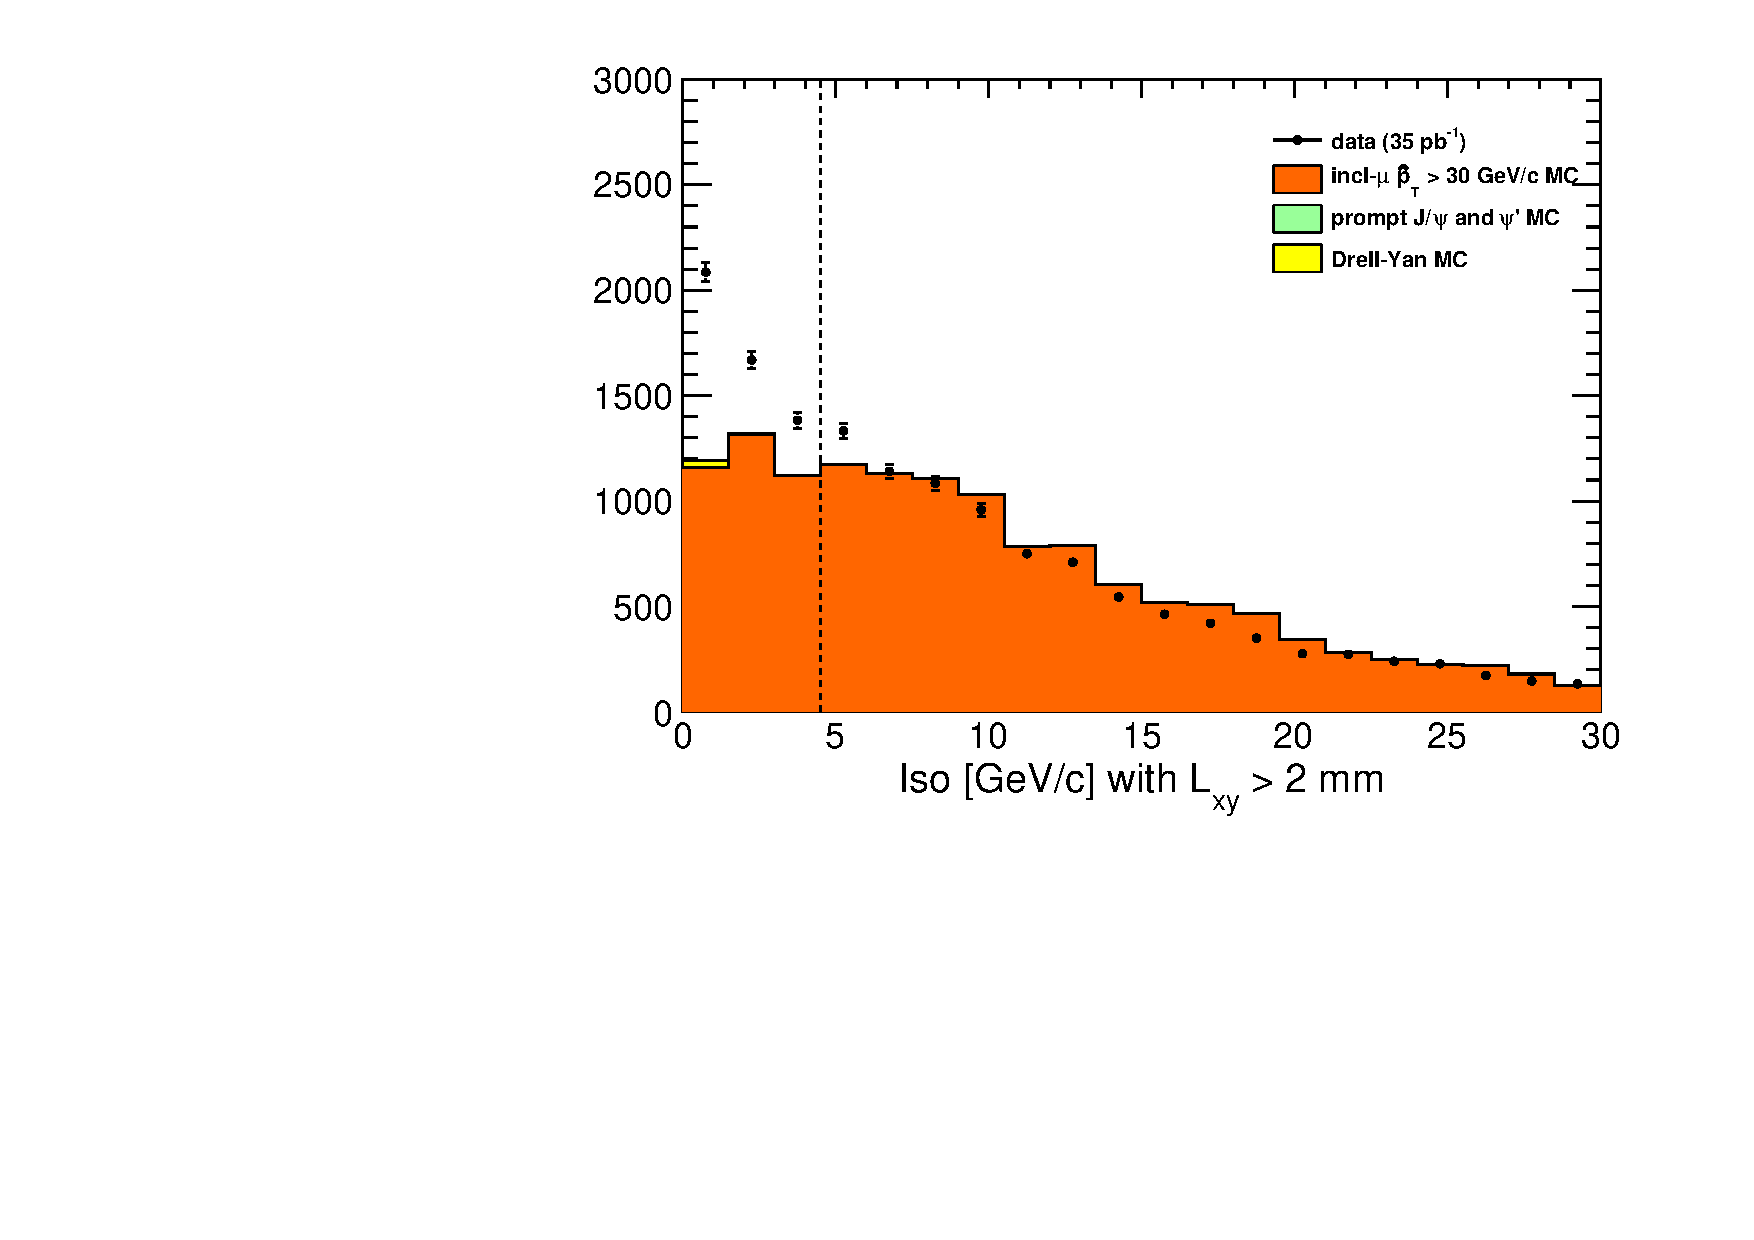
\includegraphics[width=0.5\linewidth]{lowdimuon_iso_everything2.pdf}
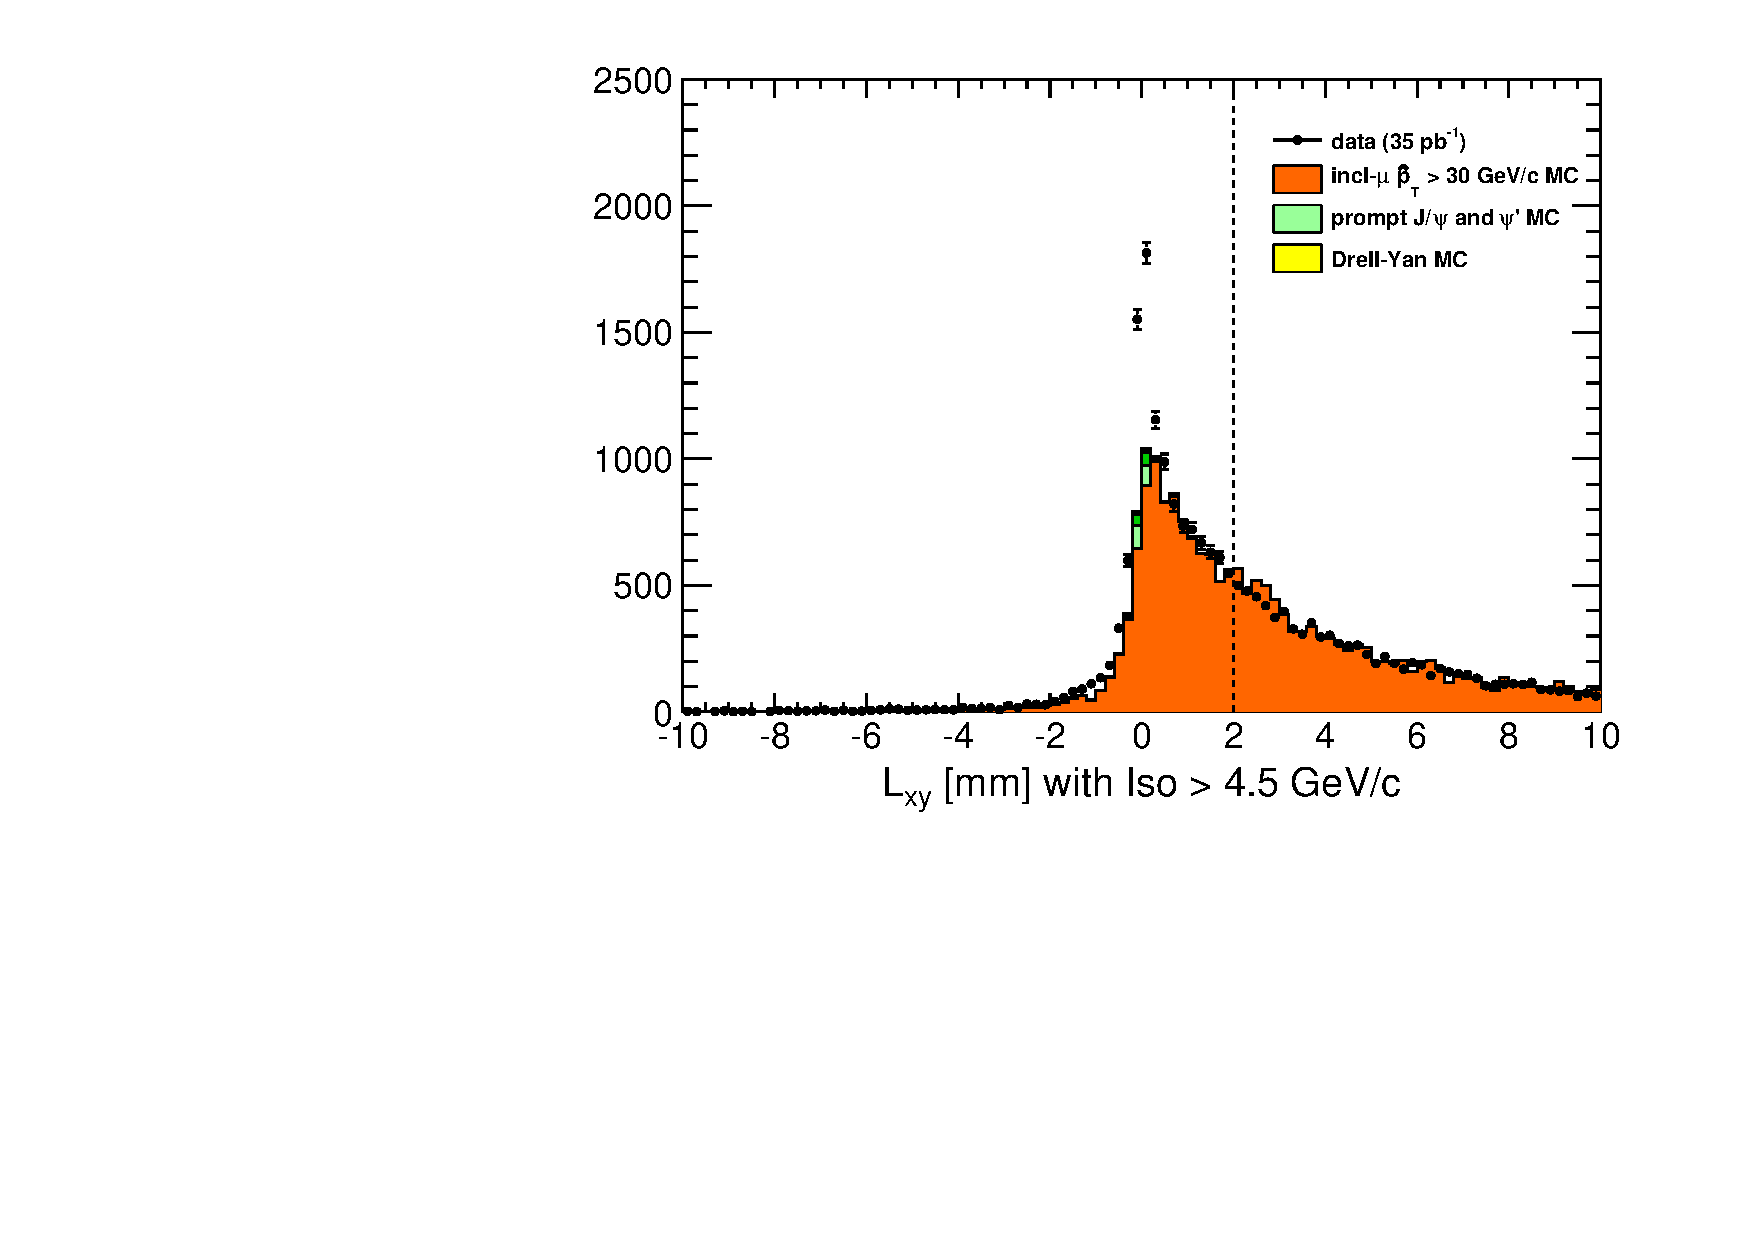
\includegraphics[width=0.5\linewidth]{lowdimuon_lxy_everything2.pdf}
\end{frame}

\begin{frame}
\frametitle{$b\bar{b}$ cuts for mass template}

\begin{itemize}
\item Select $Iso > 4.5$~GeV/$c$ {\bf or} $L_{xy} > 2$~mm
\item Efficiency for $b \to 2\mu X$ (in incl-$\mu$ MC) is $\sim$90\% and uniform in mass
\end{itemize}

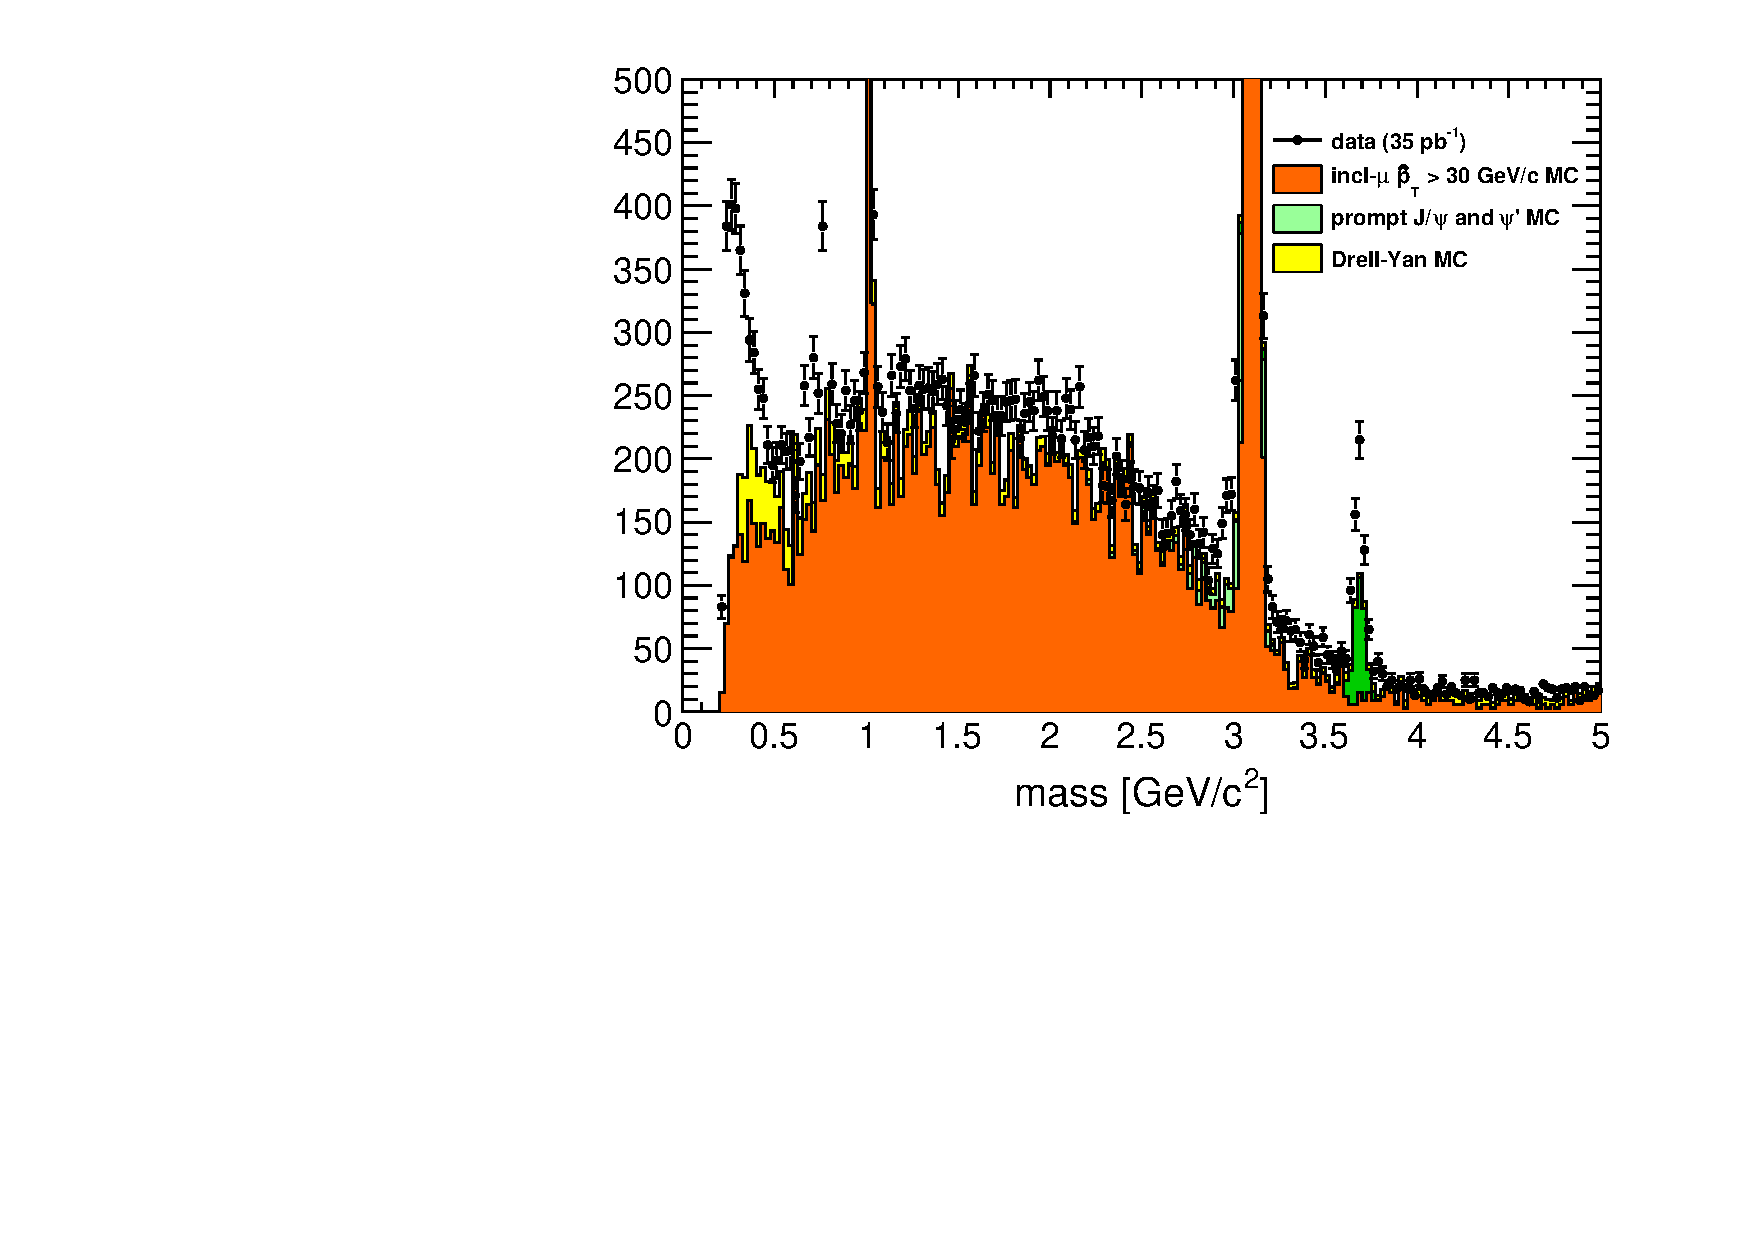
\includegraphics[width=0.5\linewidth]{lowdimuon_mass_nobcuts.pdf}
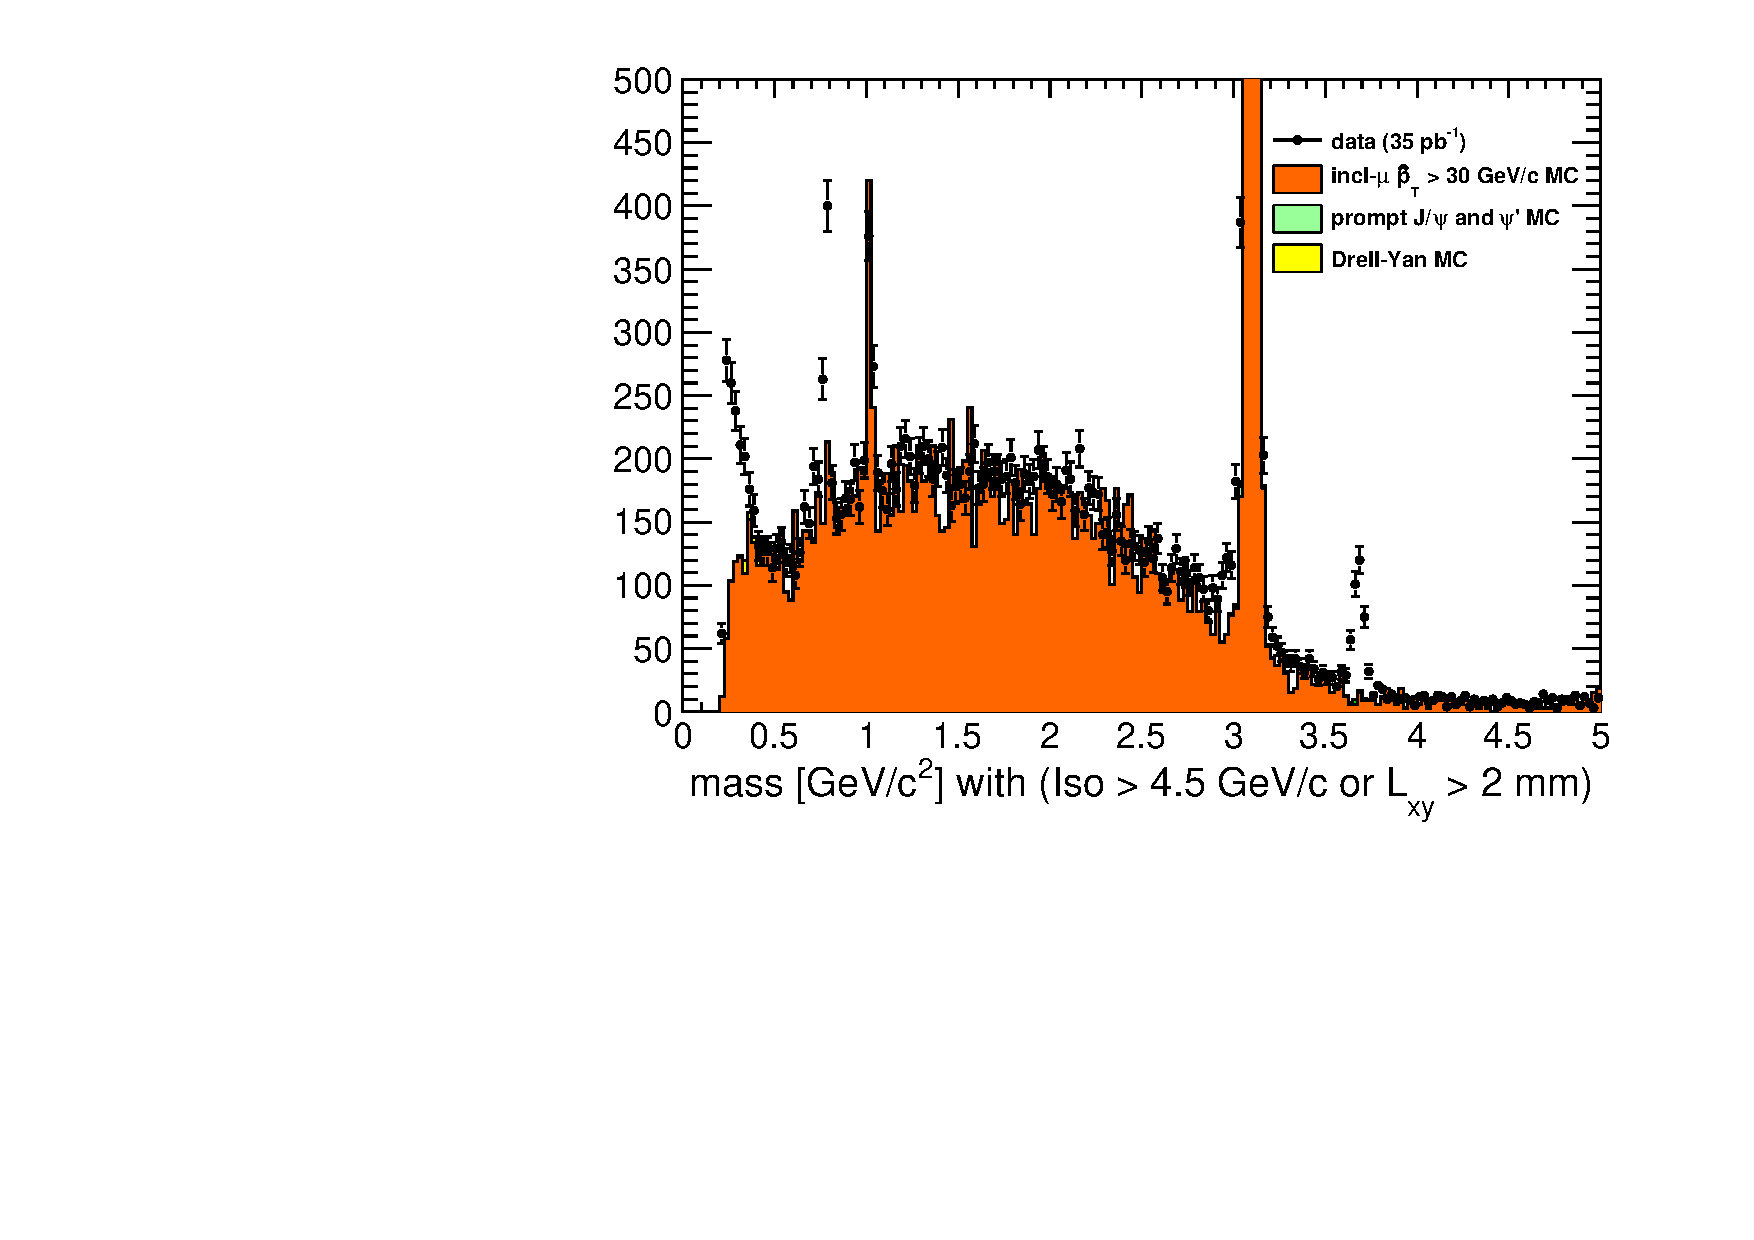
\includegraphics[width=0.5\linewidth]{lowdimuon_mass_bcuts.pdf}
\begin{center}
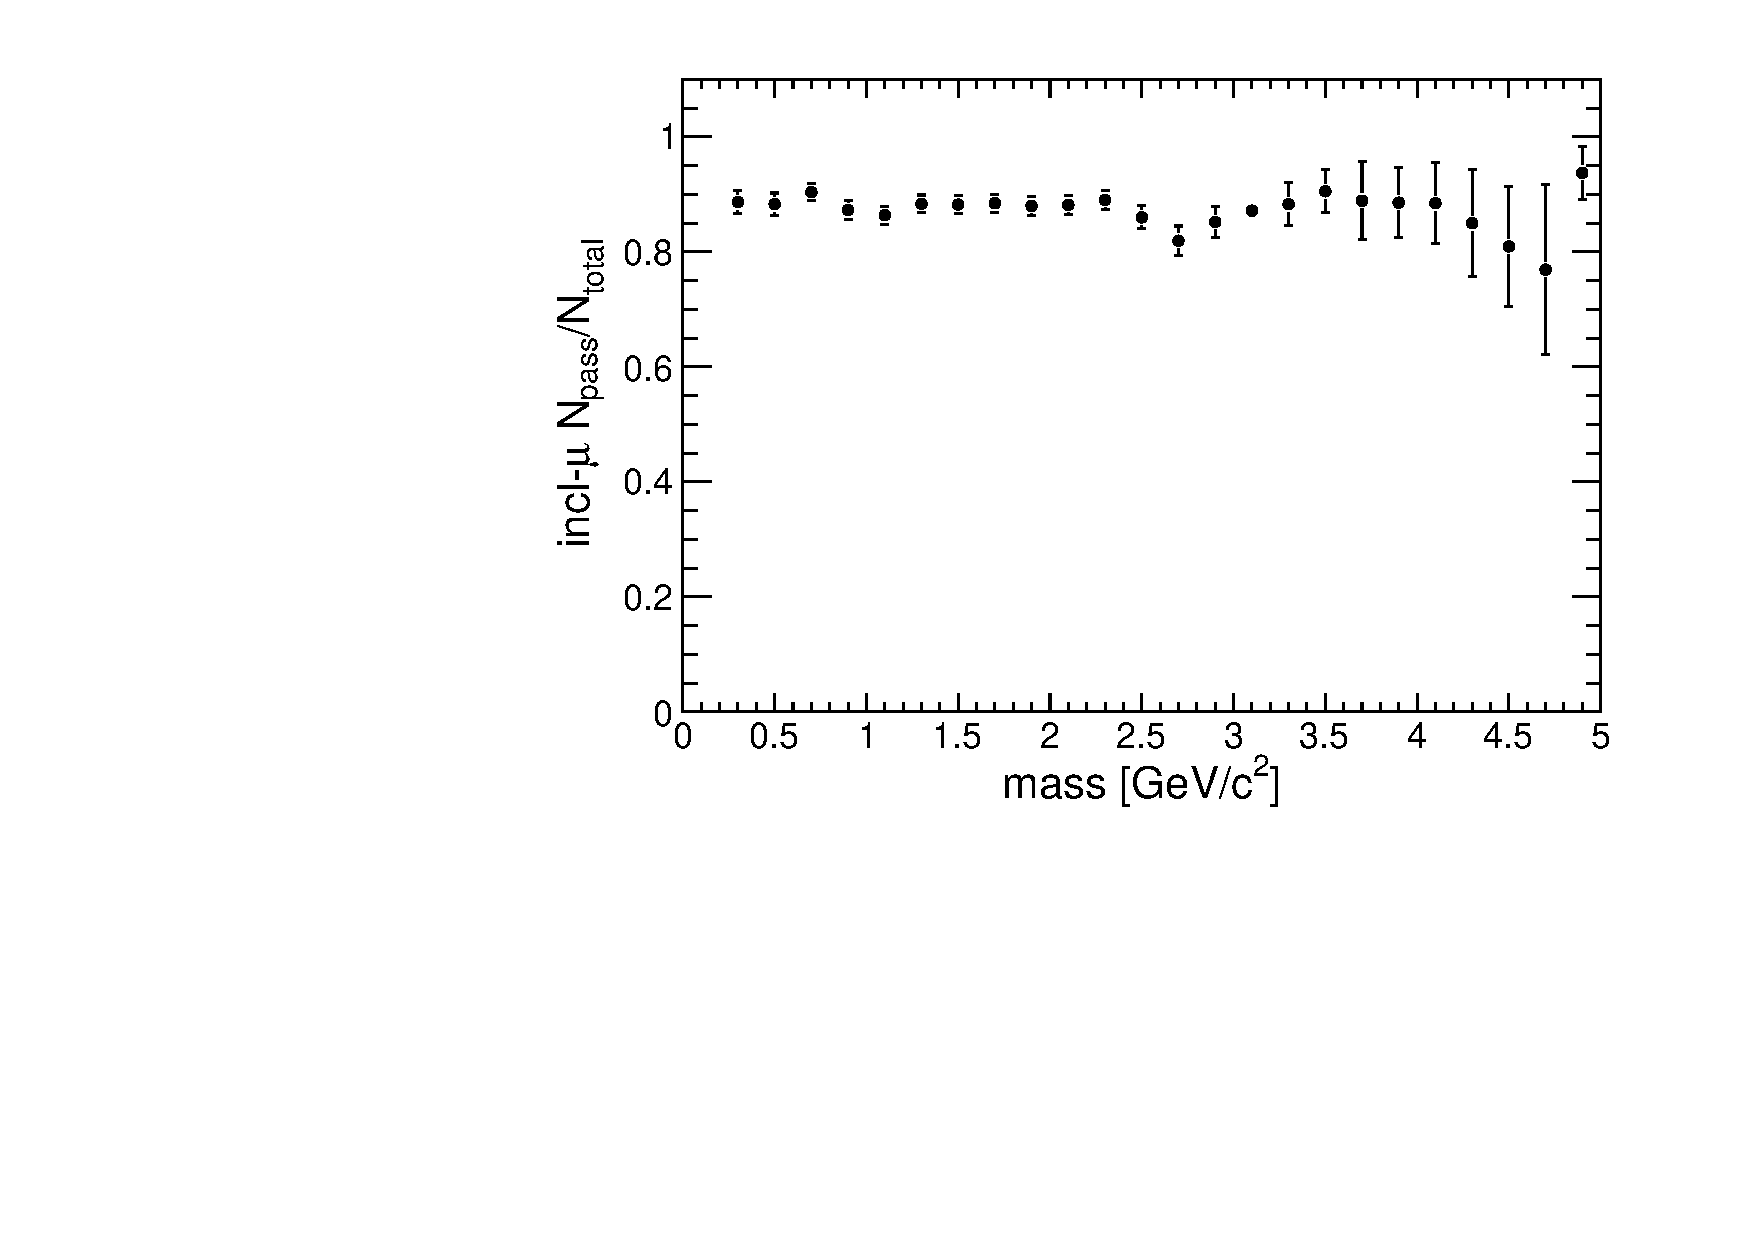
\includegraphics[width=0.45\linewidth]{lowdimuon_mass_bcut_efficiency.pdf}
\end{center}
\end{frame}

\begin{frame}
\frametitle{Dimuon-dimuon mass template}

\begin{itemize}
\item Can either get a histogram from the FitNtuple:

{\tt \tiny tfile.Get("FitNtuple/lowdimuon").Draw("mass", "muontrigpt > 12. \&\& (iso > 4.5 || ((pluspx+minuspx)*vx + (pluspy+minuspy)*vy)/sqrt((pluspx+minuspx)**2 + (pluspy+minuspy)**2) > 0.2)")}

\item Or use this parameterized shape for smoothness:

{\tt \tiny 289.65*exp(-(x-0.78265)**2 / 2. / 0.011**2) + 214.63*exp(-(x-1.019455)**2 / 2. / 0.014**2) + 2753.22*exp(-(x-3.096916)**2 / 2. / 0.025**2) + 93.04*exp(-(x-3.68609)**2 / 2. / 0.029**2) + 30.59/(x-2.*0.105658367) + 2.31 + 9.01*(x-5) + -10.87*(x-5)**2 + -25.15*(x-5)**3 + -4.92*(x-5)**4}

\item Taken from a fit to single dimuon data with the $b$-cut:
\end{itemize}
\begin{center}
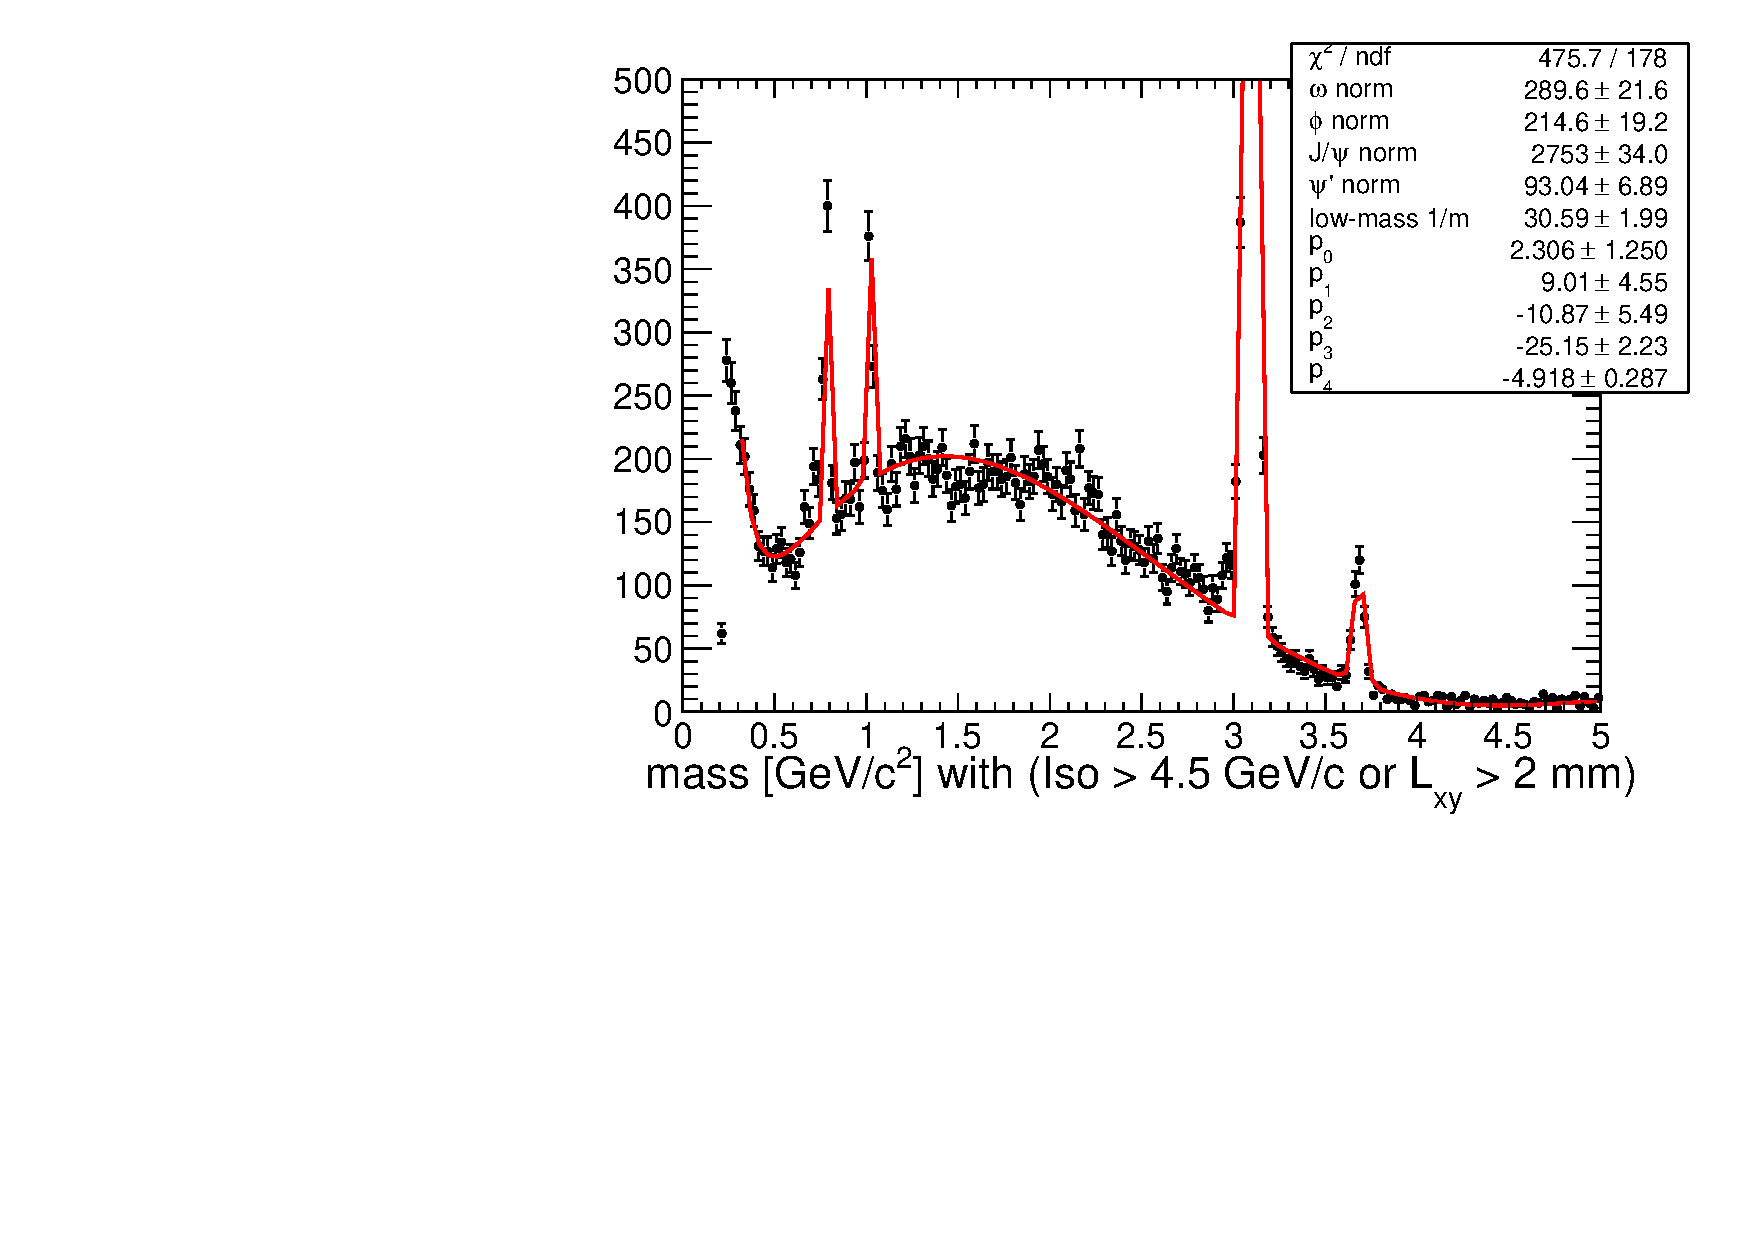
\includegraphics[width=0.5\linewidth]{lowdimuon_mass_bcuts_backgroundfit_zoom.pdf}
\end{center}
\end{frame}

\begin{frame}
\frametitle{Single dimuon mass template}

\begin{itemize}
\item For the ``single $p_T > 80$~GeV/$c$ dimuon'' signal channel, we
  should not exclude the isolated, $L_{xy} \sim 0$ part of the distribution
  (Drell-Yan can contribute to {\it this} signal region)
\item We should, however, find derive the template from a part of the
  spectrum where the two contributions scale the same way in $p_T$
  (that is, get away from turn-on curves and prompt production)
\item For $40 < p_T < 80$~GeV/$c$, the ratio is flat: we {\it assume} it is still flat for $p_T > 80$~GeV/$c$, since this is far away from any relevant scales
\end{itemize}

\begin{center}
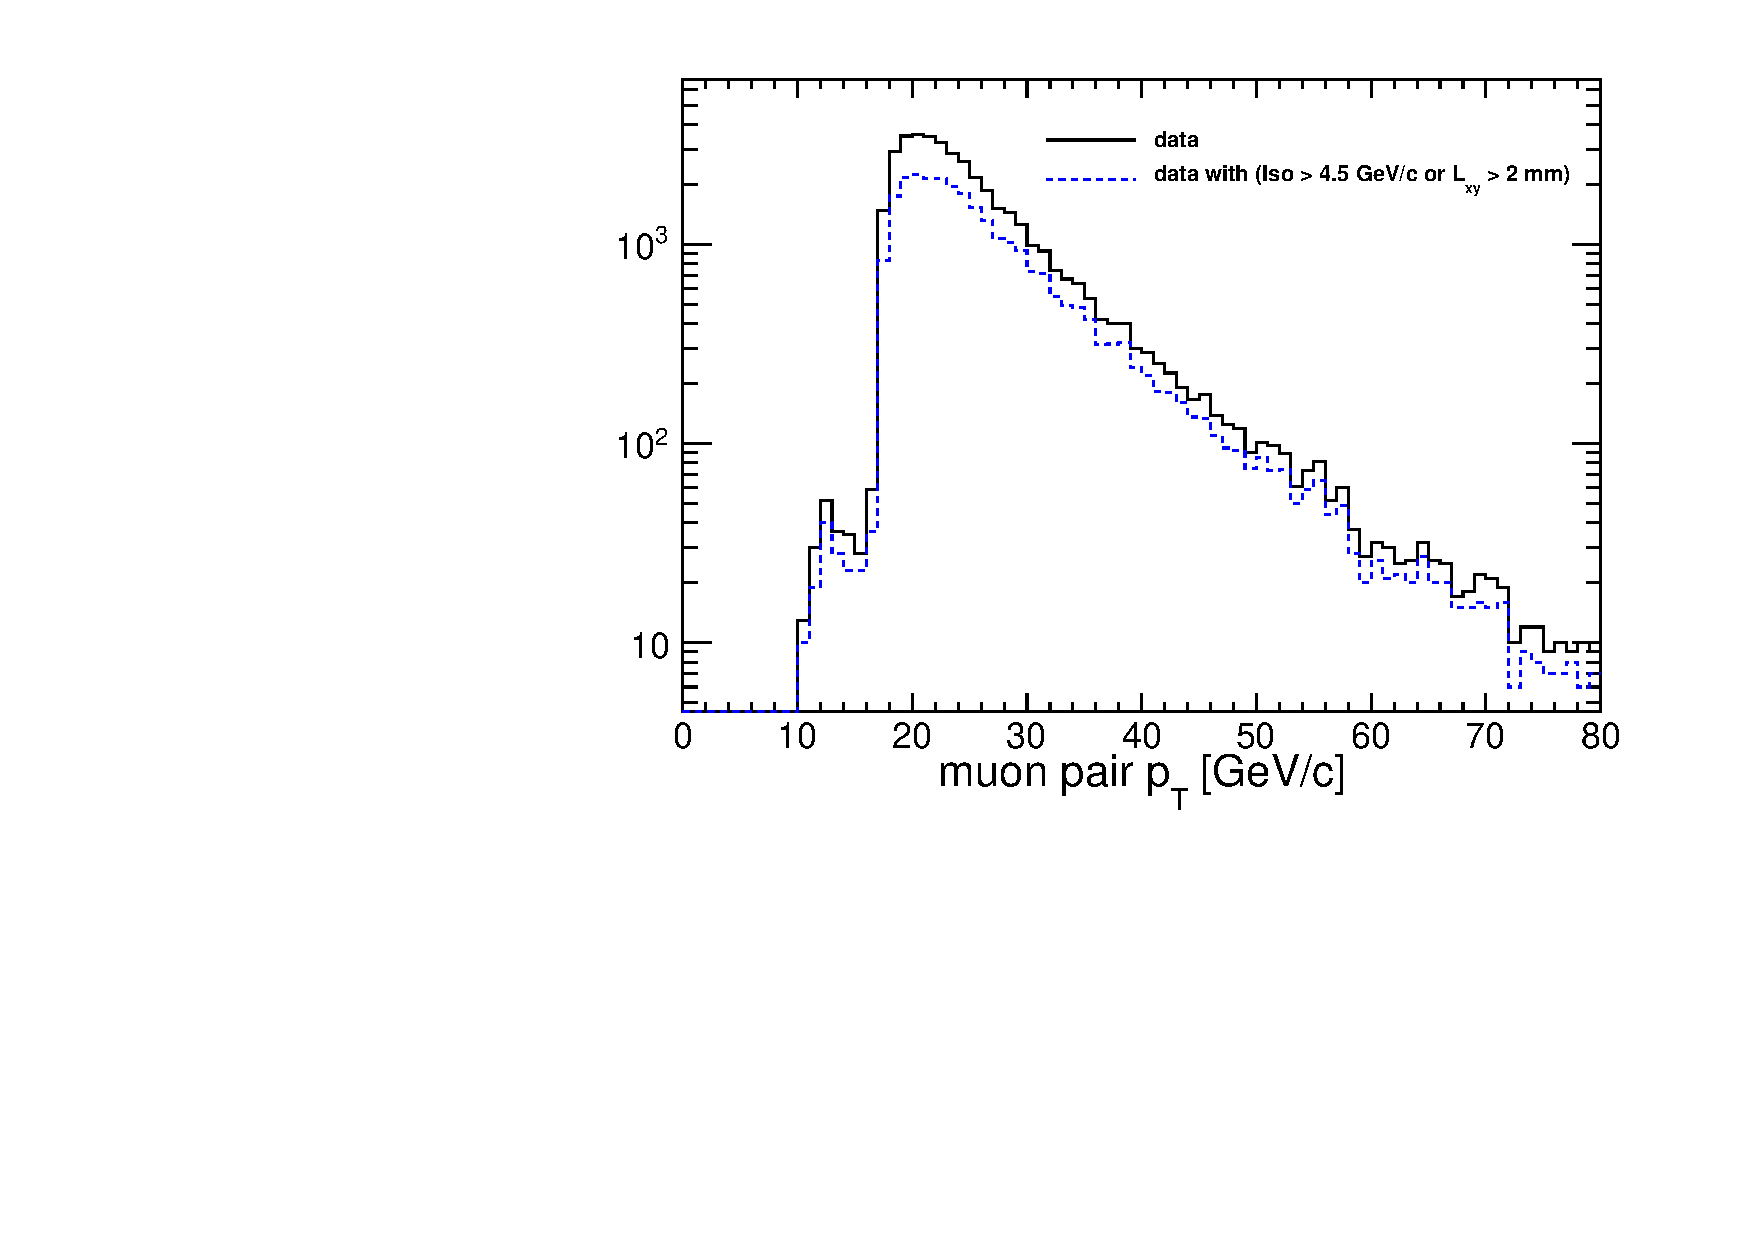
\includegraphics[width=0.5\linewidth]{lowdimuon_40-80_distributions.pdf}
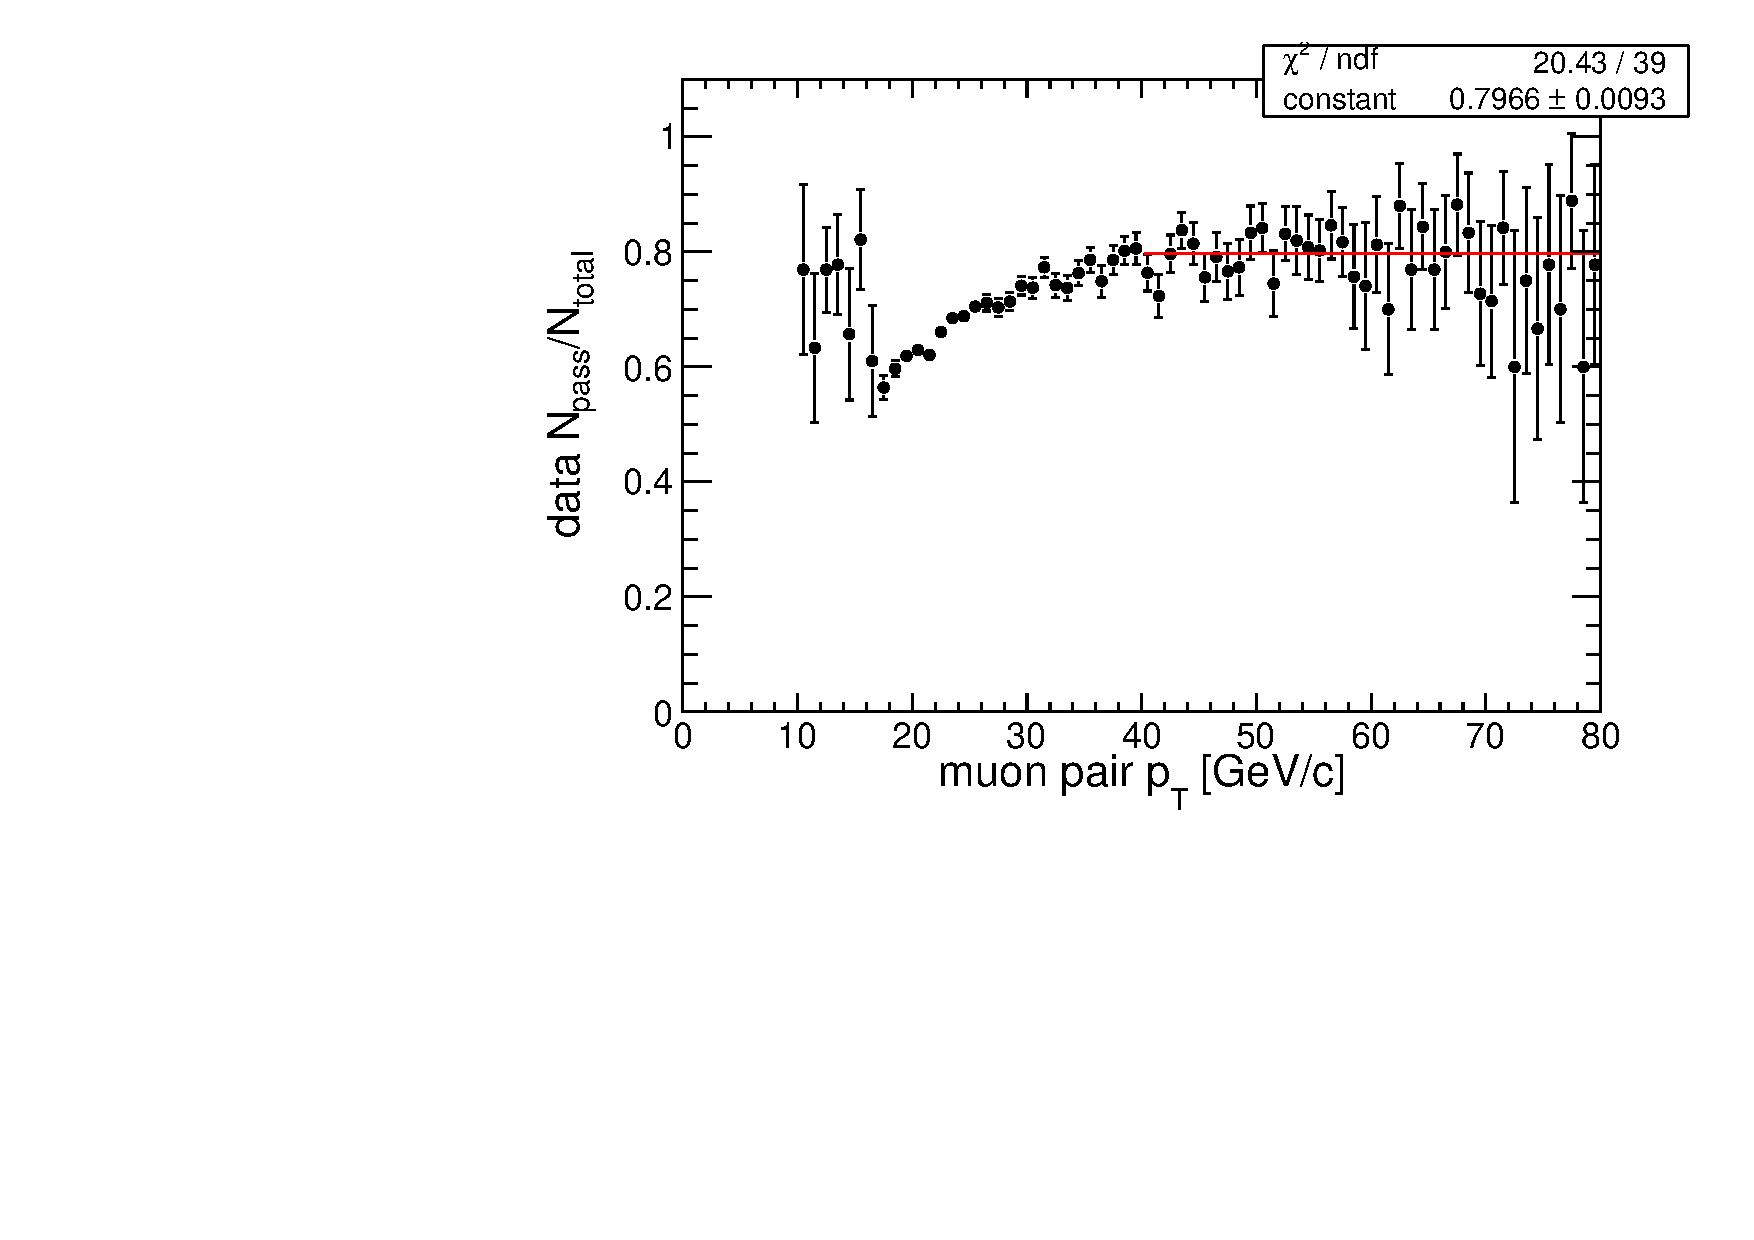
\includegraphics[width=0.5\linewidth]{lowdimuon_40-80_ratio.pdf}
\end{center}
\end{frame}

\begin{frame}
\frametitle{Single dimuon mass template}

\begin{itemize}
\item \textcolor{gray}{For the ``single $p_T > 80$~GeV/$c$ dimuon'' signal channel, we
  should not exclude the isolated, $L_{xy} \sim 0$ part of the distribution
  (Drell-Yan can contribute to {\it this} signal region)}
\item \textcolor{gray}{We should, however, find derive the template from a part of the
  spectrum where the two contributions scale the same way in $p_T$
  (that is, get away from turn-on curves and prompt production)}
\item The ratio is not flat in mass, but this is because $b\bar{b}$
  contributes to a different part of the spectrum than Drell-Yan.  We
  want both.
\end{itemize}

\begin{center}
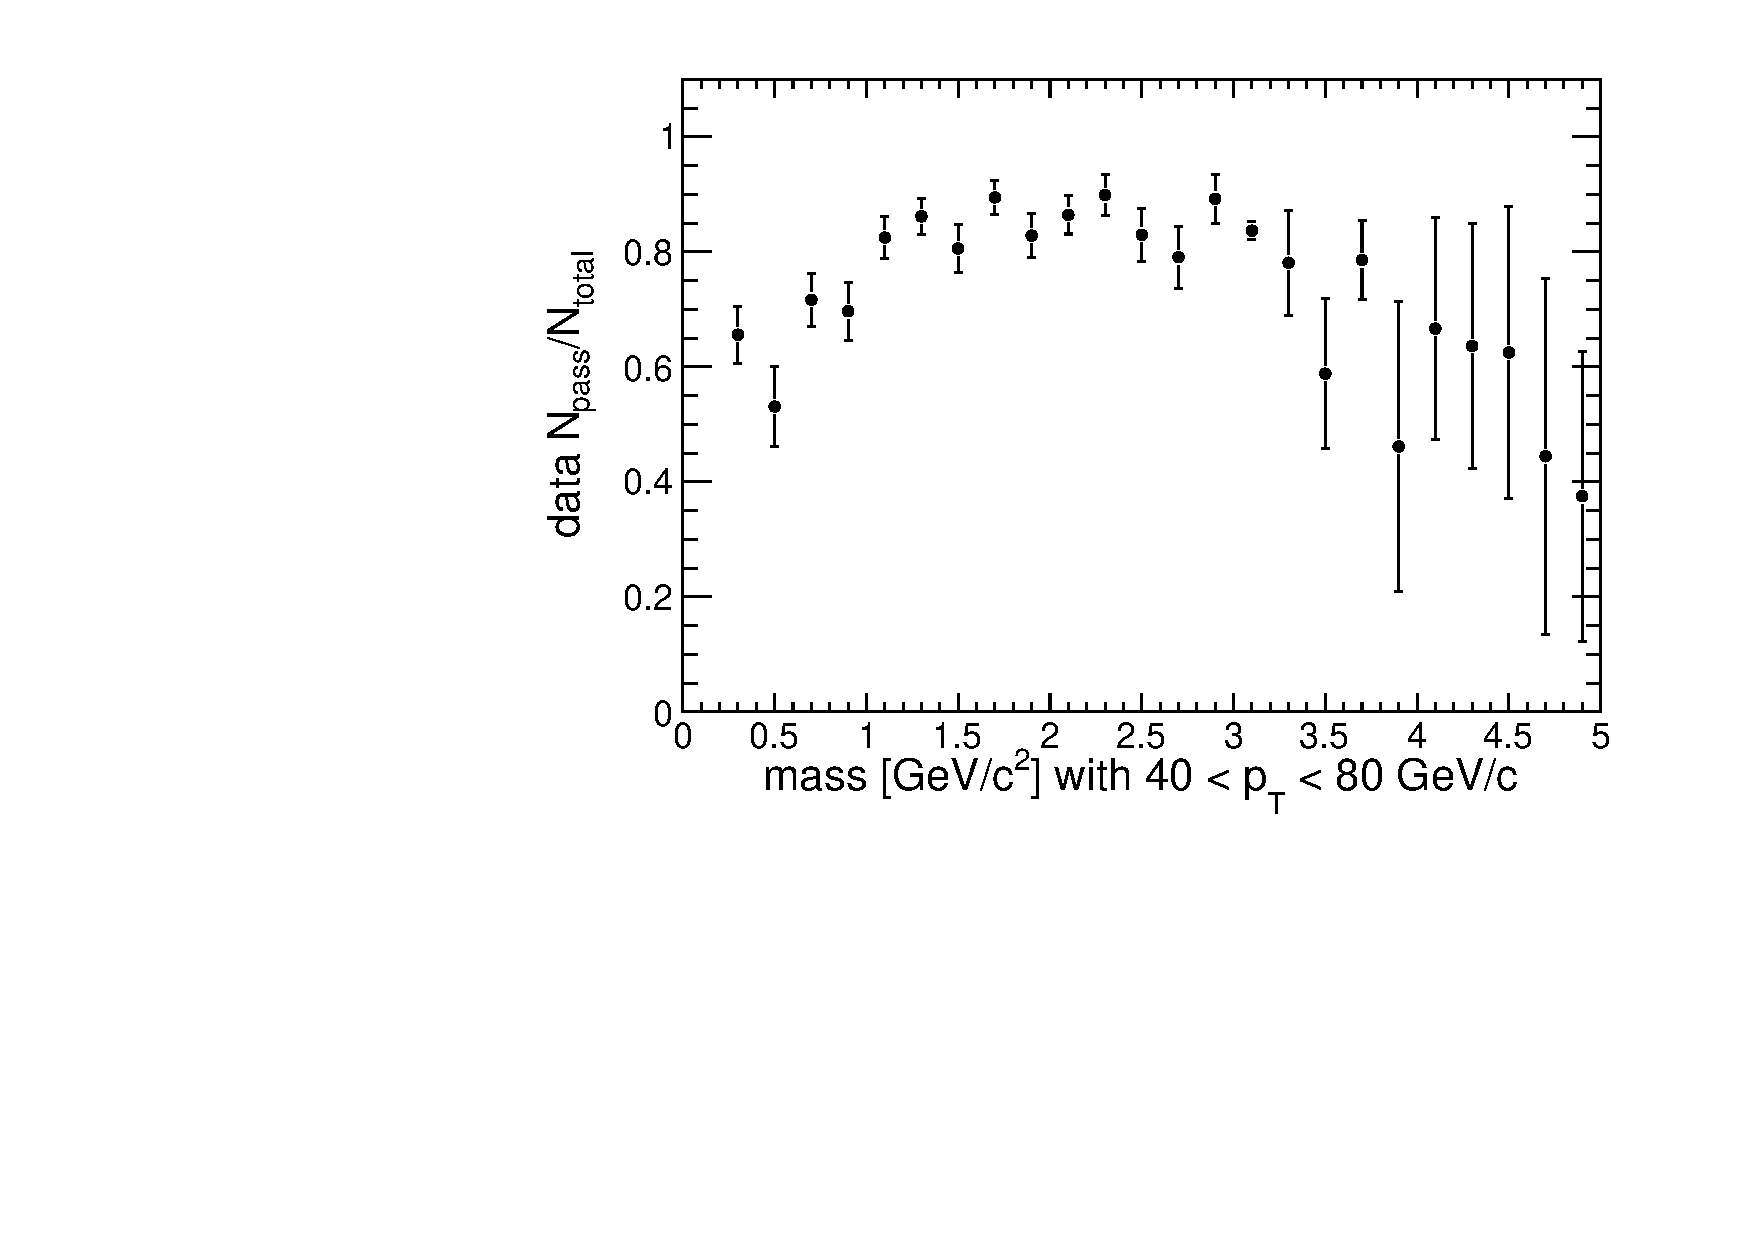
\includegraphics[width=0.5\linewidth]{lowdimuon_40-80_massratio.pdf}
\end{center}
\end{frame}

\begin{frame}
\frametitle{Single dimuon mass template}

\begin{itemize}
\item Can either get a histogram from the FitNtuple:

{\tt \tiny tfile.Get("FitNtuple/lowdimuon").Draw("mass", "muontrigpt > 12. \&\& 40. < pt \&\& pt < 80.")}

\item Or use this parameterized shape for smoothness:

{\tt \tiny 20.36*exp(-(x-0.78265)**2 / 2. / 0.011**2) + 14.86*exp(-(x-1.019455)**2 / 2. / 0.014**2) + 271.55*exp(-(x-3.096916)**2 / 2. / 0.025**2) + 8.93*exp(-(x-3.68609)**2 / 2. / 0.029**2) + 3.13/(x-2.*0.105658367) + 0.83 + 0.37*(x-5) + -1.02*(x-5)**2 + -1.82*(x-5)**3 + -0.34*(x-5)**4}

\item Taken from a fit to single dimuon data with $40 < p_T < 80$~GeV/$c$:
\end{itemize}
\begin{center}
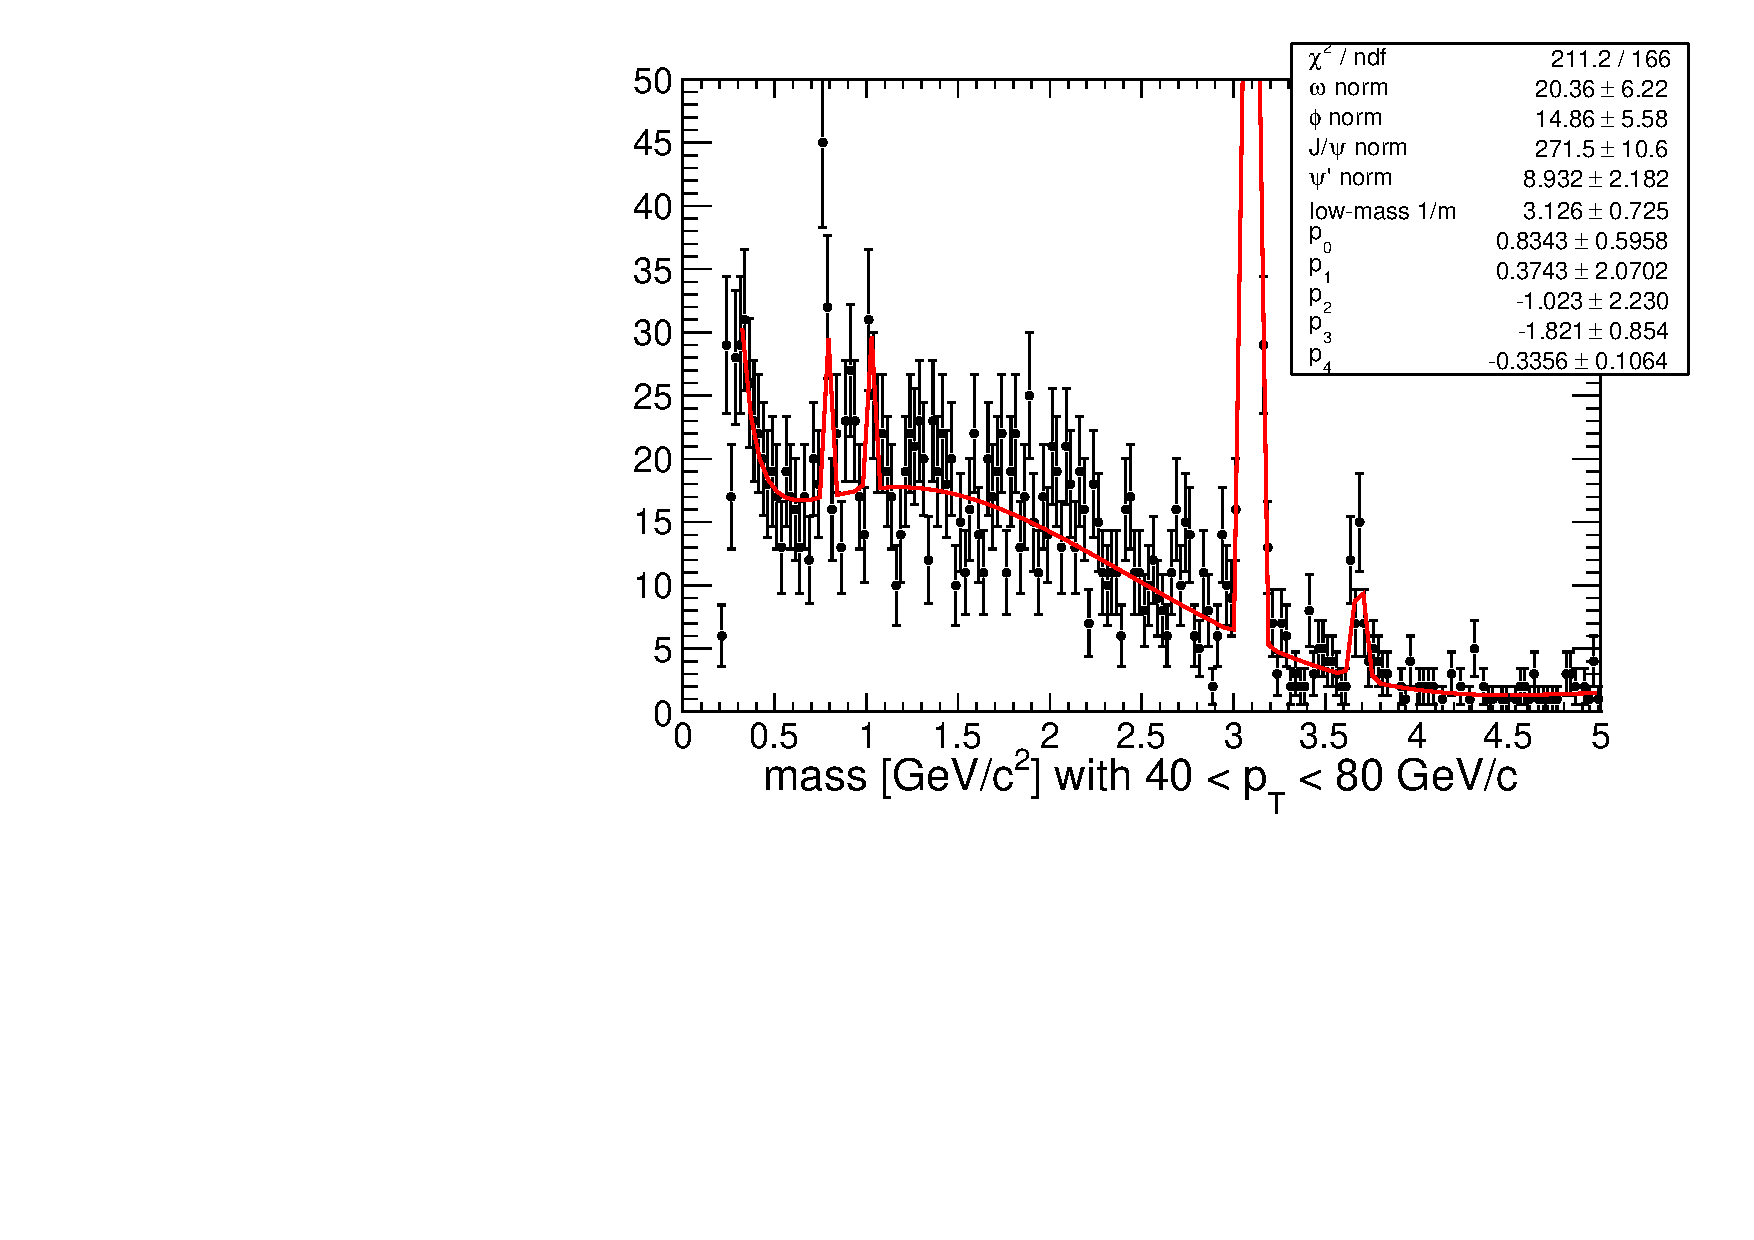
\includegraphics[width=0.5\linewidth]{lowdimuon_40-80_backgroundfit_zoom.pdf}
\end{center}
\end{frame}

\begin{frame}
\frametitle{Mass resolution}

\begin{itemize}
\item Fit our four ``standard candle mu-jets'' for detector resolution {\scriptsize (masses fixed to PDG, width of $\rho$ fixed to PDG, $J/\psi$ has FSR (Crystal Ball $\alpha$) but simpler backgrounds)}
\end{itemize}

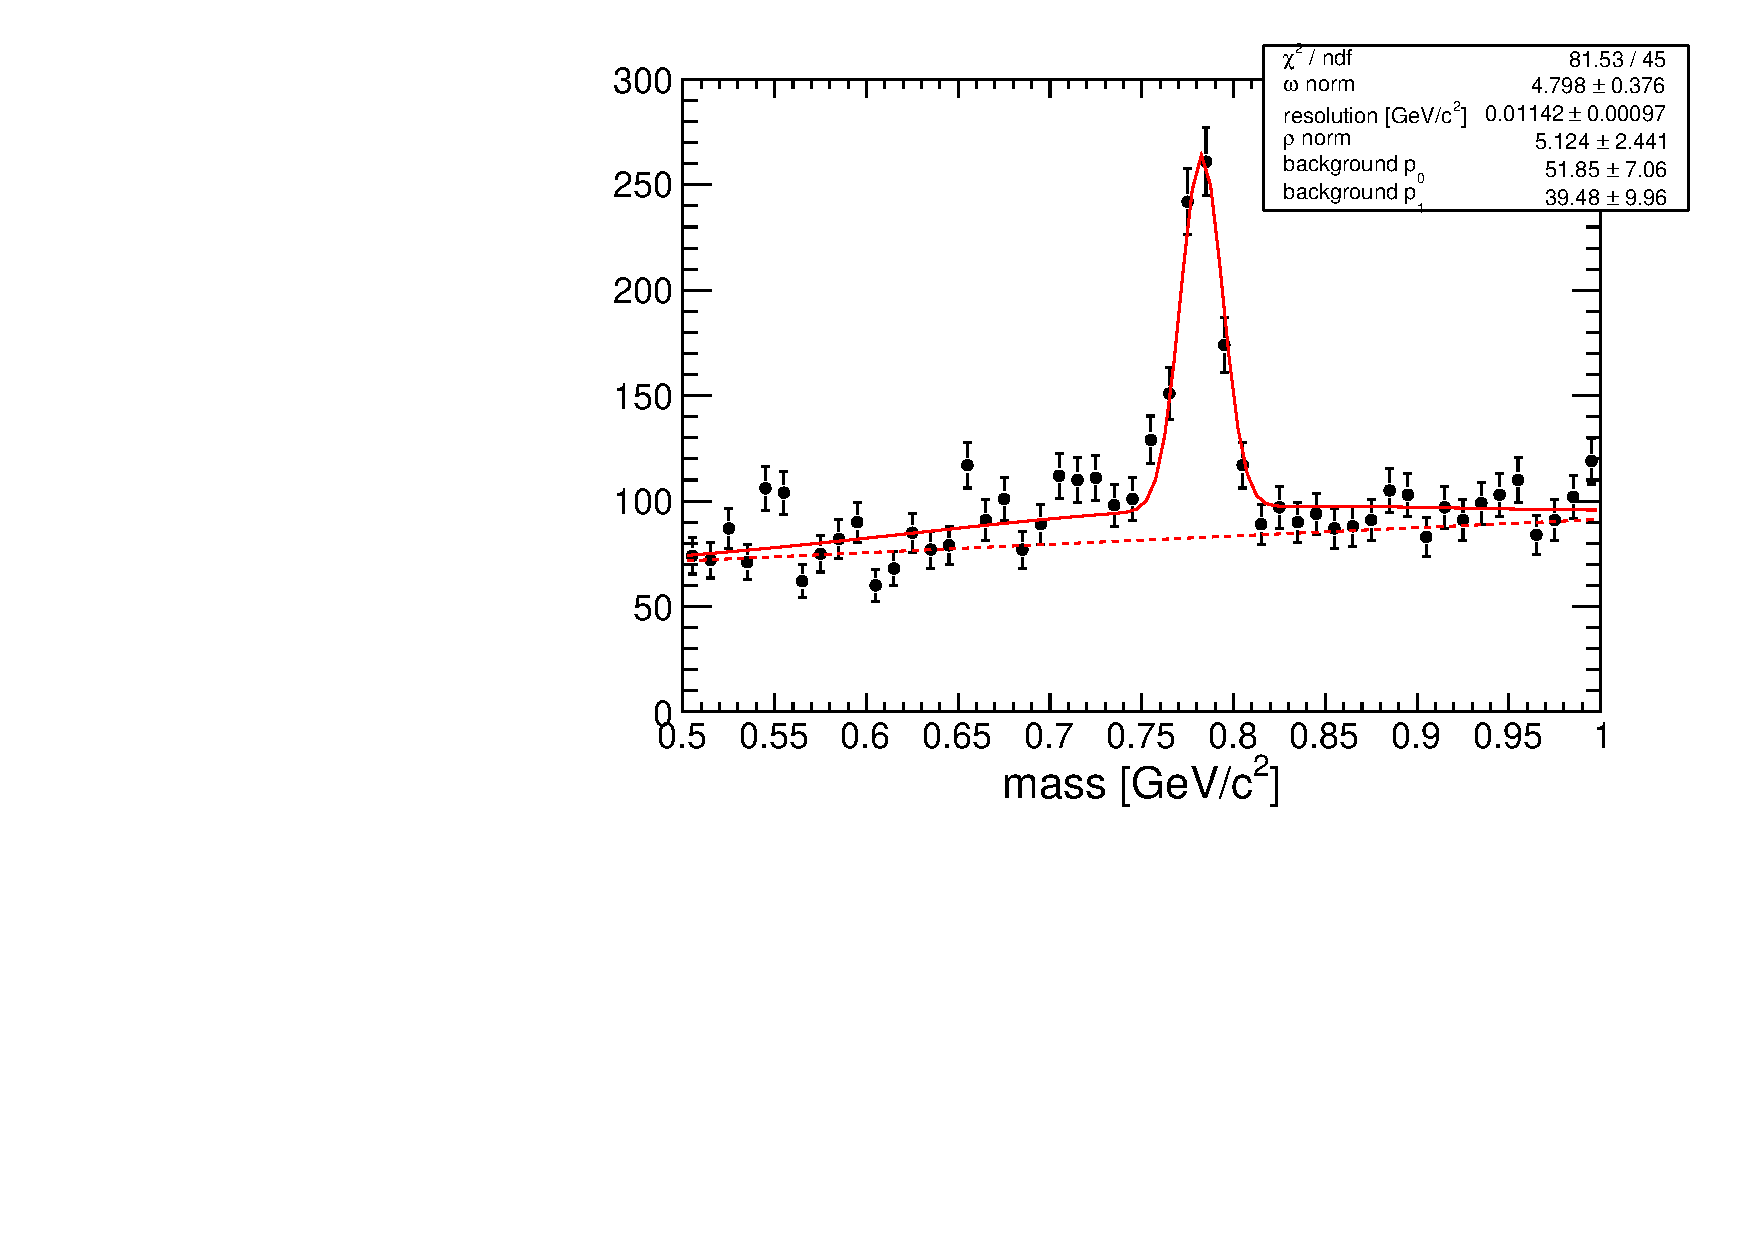
\includegraphics[width=0.47\linewidth]{respeak_omega.pdf}
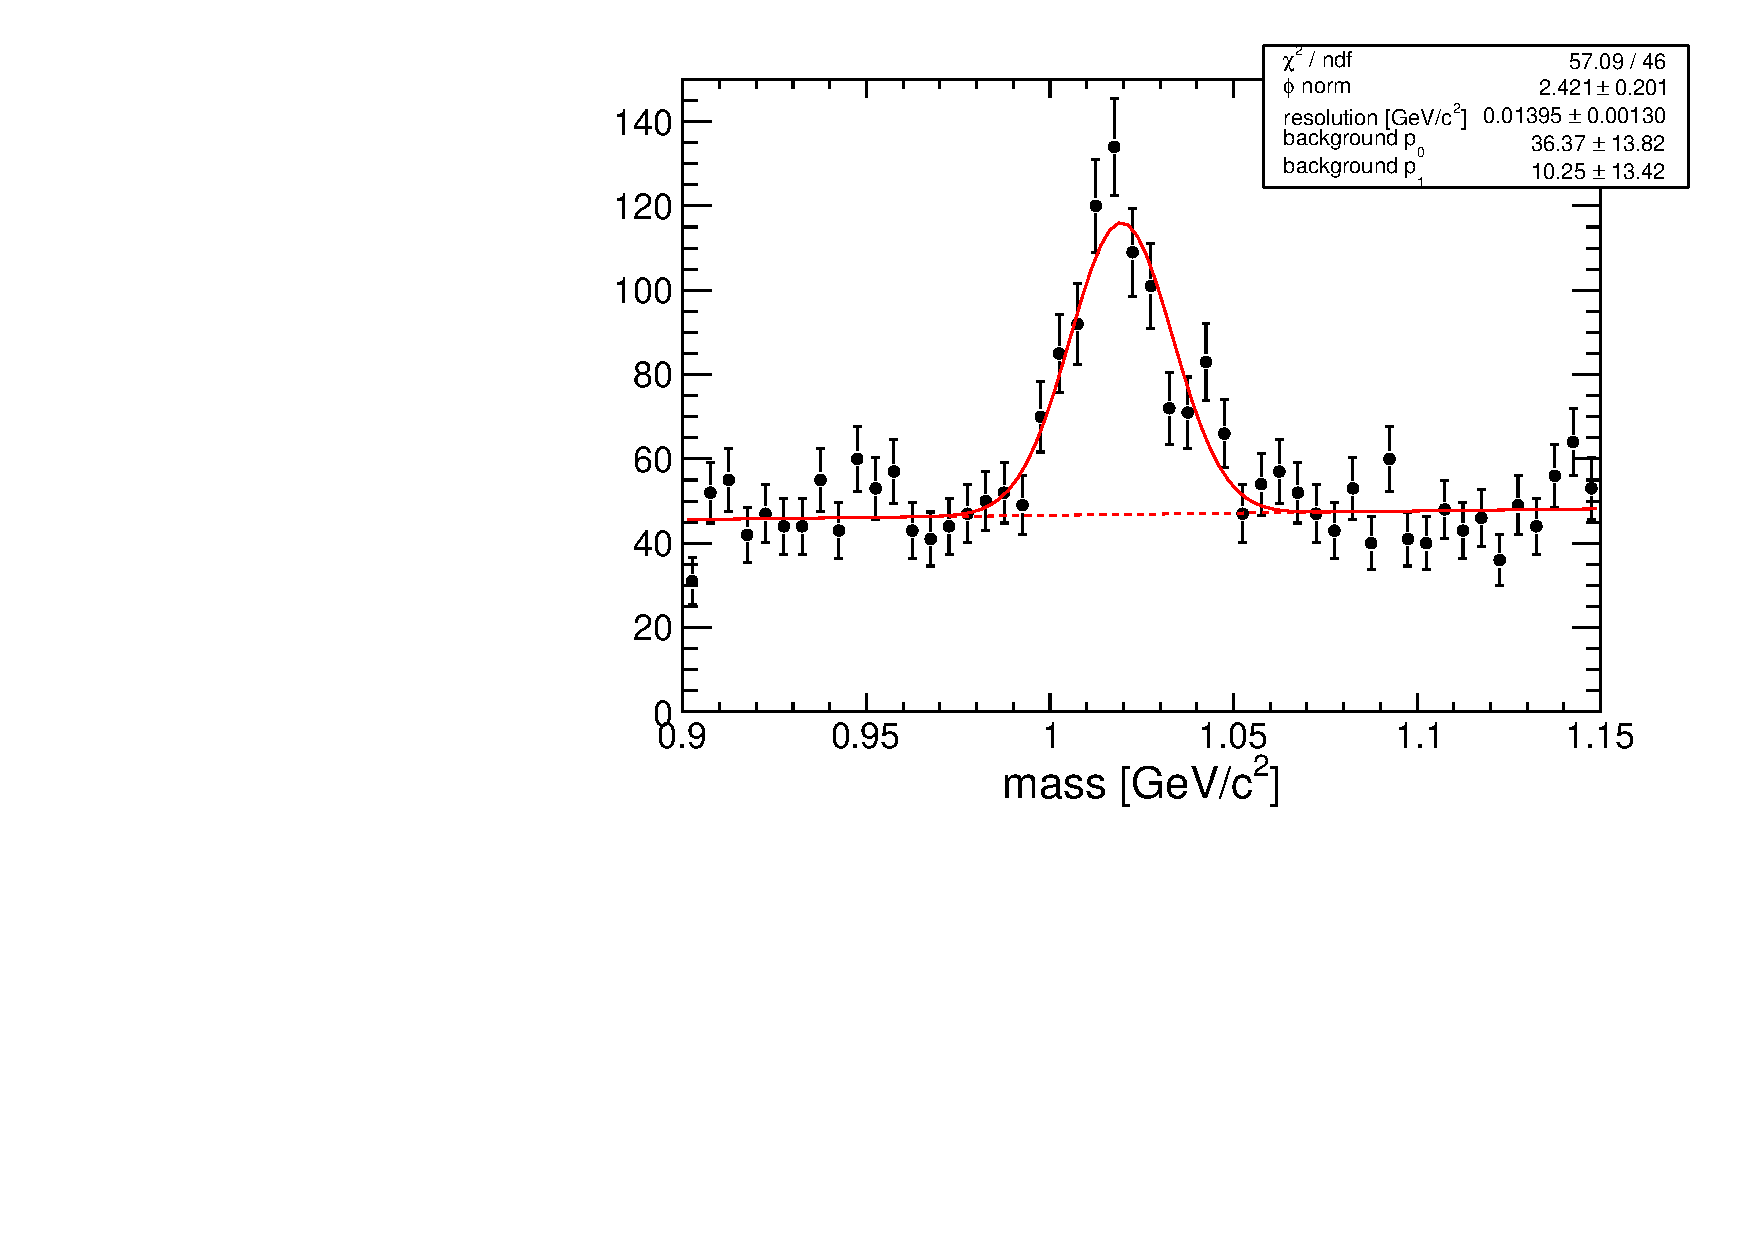
\includegraphics[width=0.47\linewidth]{respeak_phi.pdf}

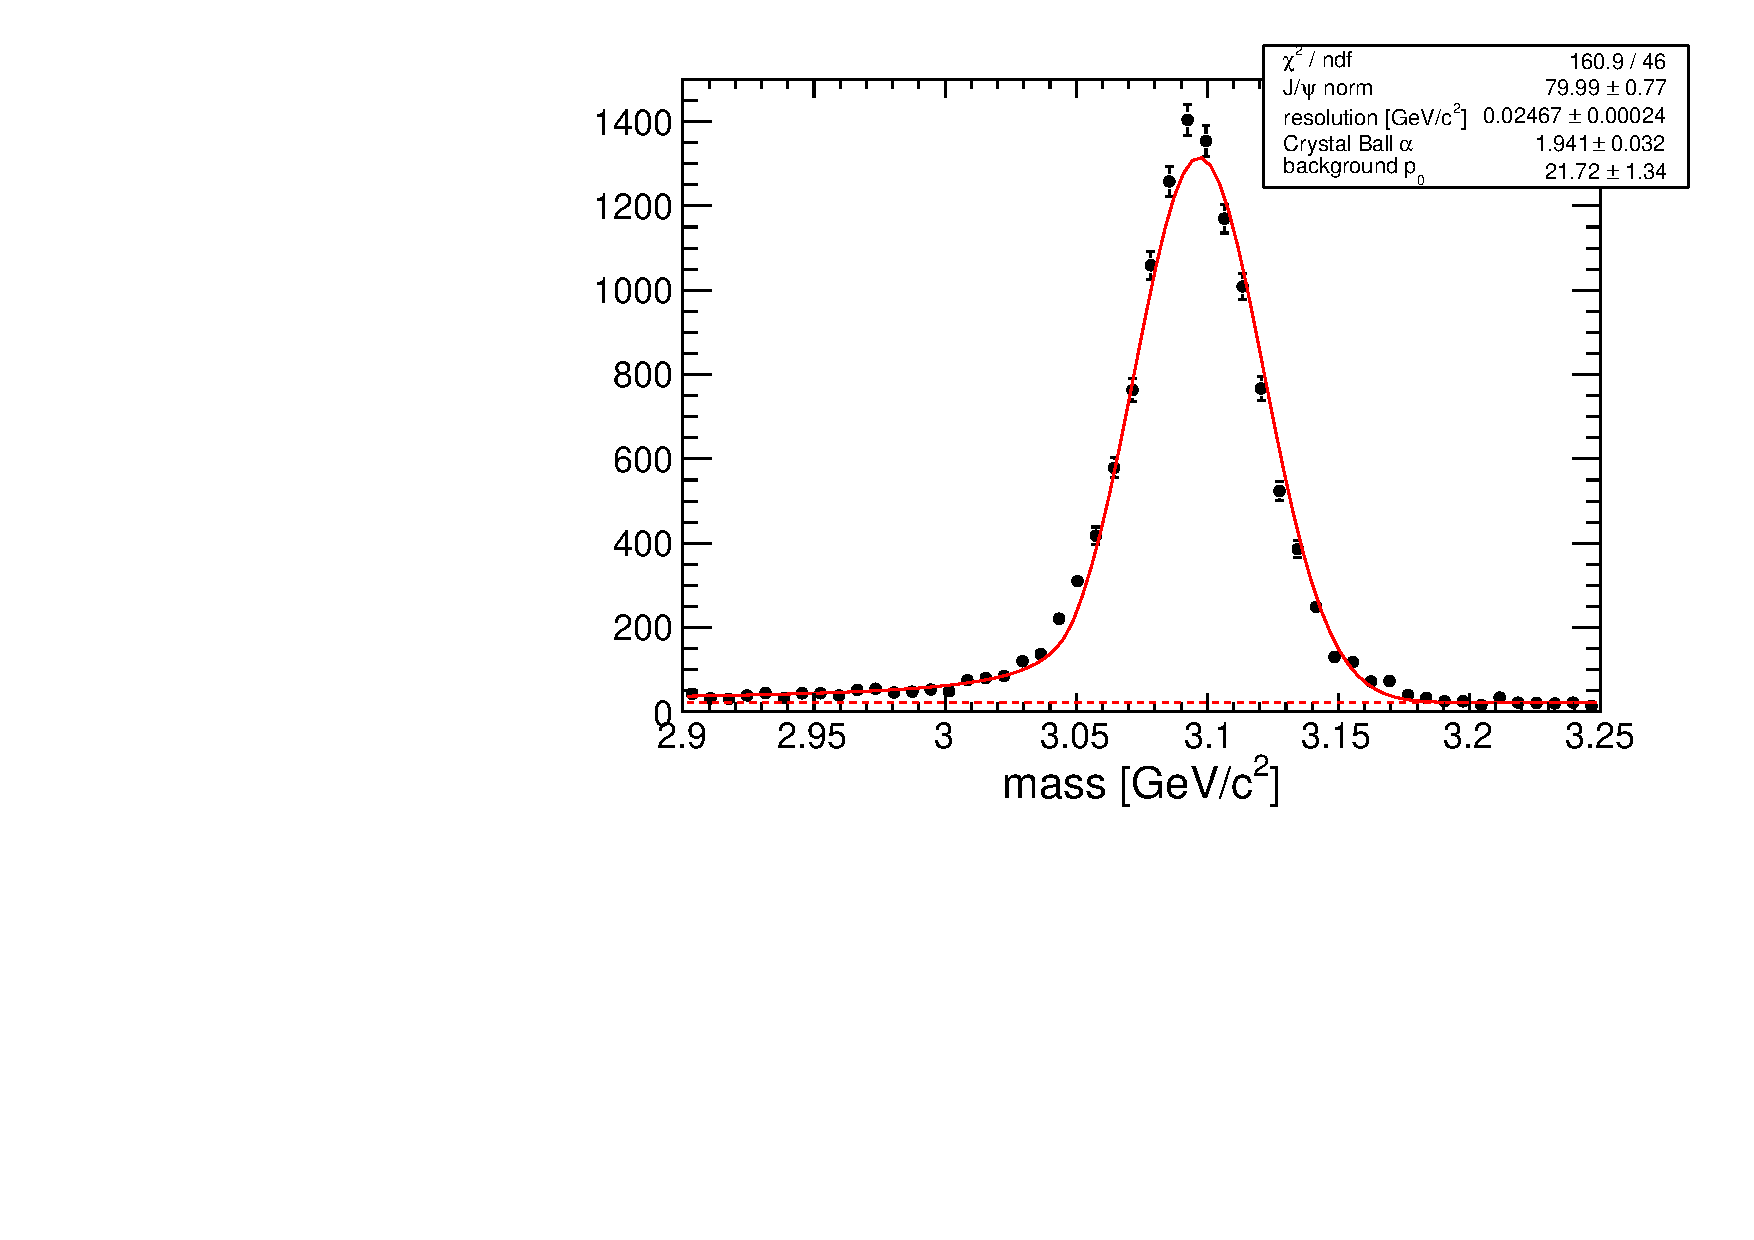
\includegraphics[width=0.47\linewidth]{respeak_jpsi.pdf}
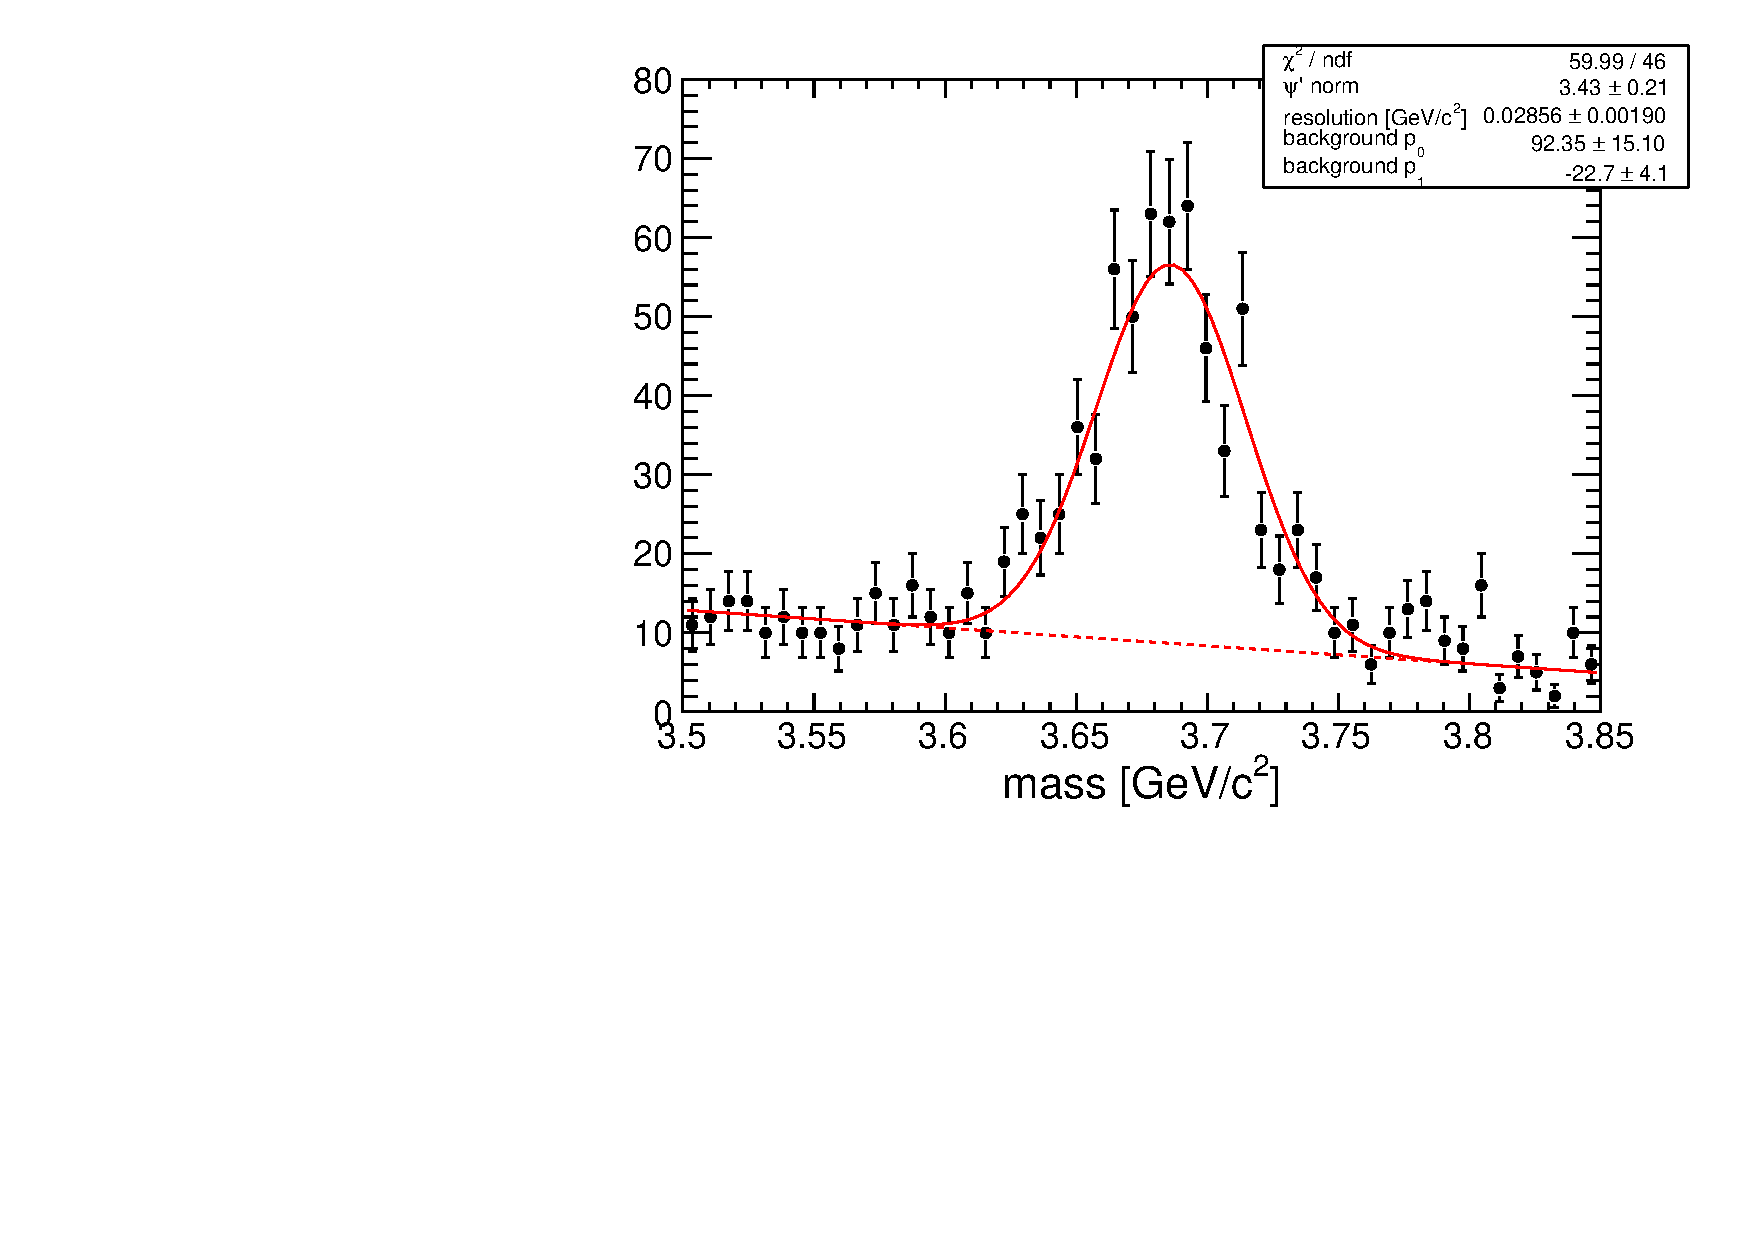
\includegraphics[width=0.47\linewidth]{respeak_psiprime.pdf}
\end{frame}

\begin{frame}
\frametitle{Mass resolution}

\begin{itemize}
\item Compare to mass resolution from dimuon gun MC
\begin{itemize}
\item \scriptsize solid lines: containing a triggerable muon ($p_T > 12$~GeV/$c$, $|\eta| < 1$)
\item \scriptsize dashed lines: no special muon constraints ($p_T > 5$~GeV/$c$, $|\eta| < 2.4$)
\item \scriptsize also split by $p_T$ (slight dependence, worse resolution at higher $p_T$)
\end{itemize}

\item Most of the difference is due to allowing the endcap

\item MC has larger FSR tails (Crystal Ball $\alpha$ parameter)
\end{itemize}

\vfill
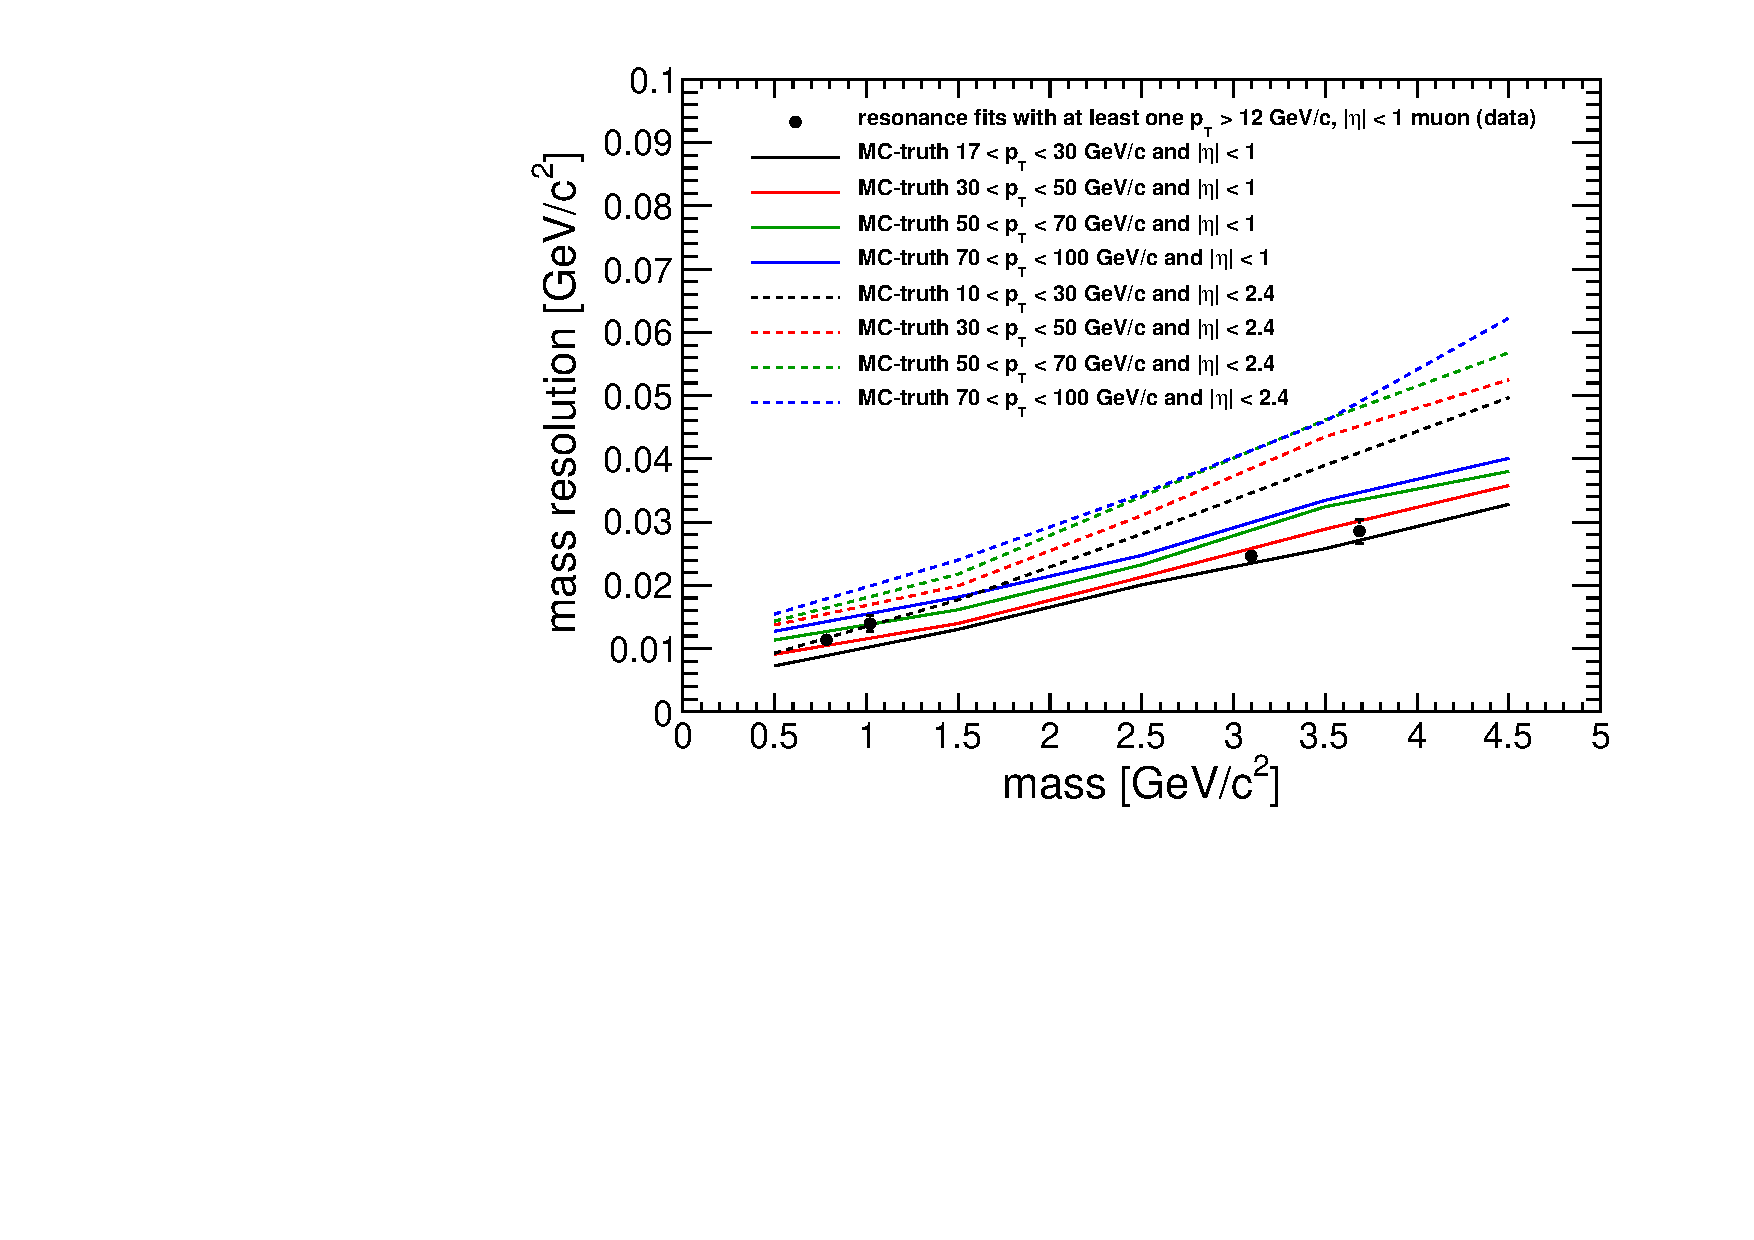
\includegraphics[width=0.5\linewidth]{resolution.pdf}
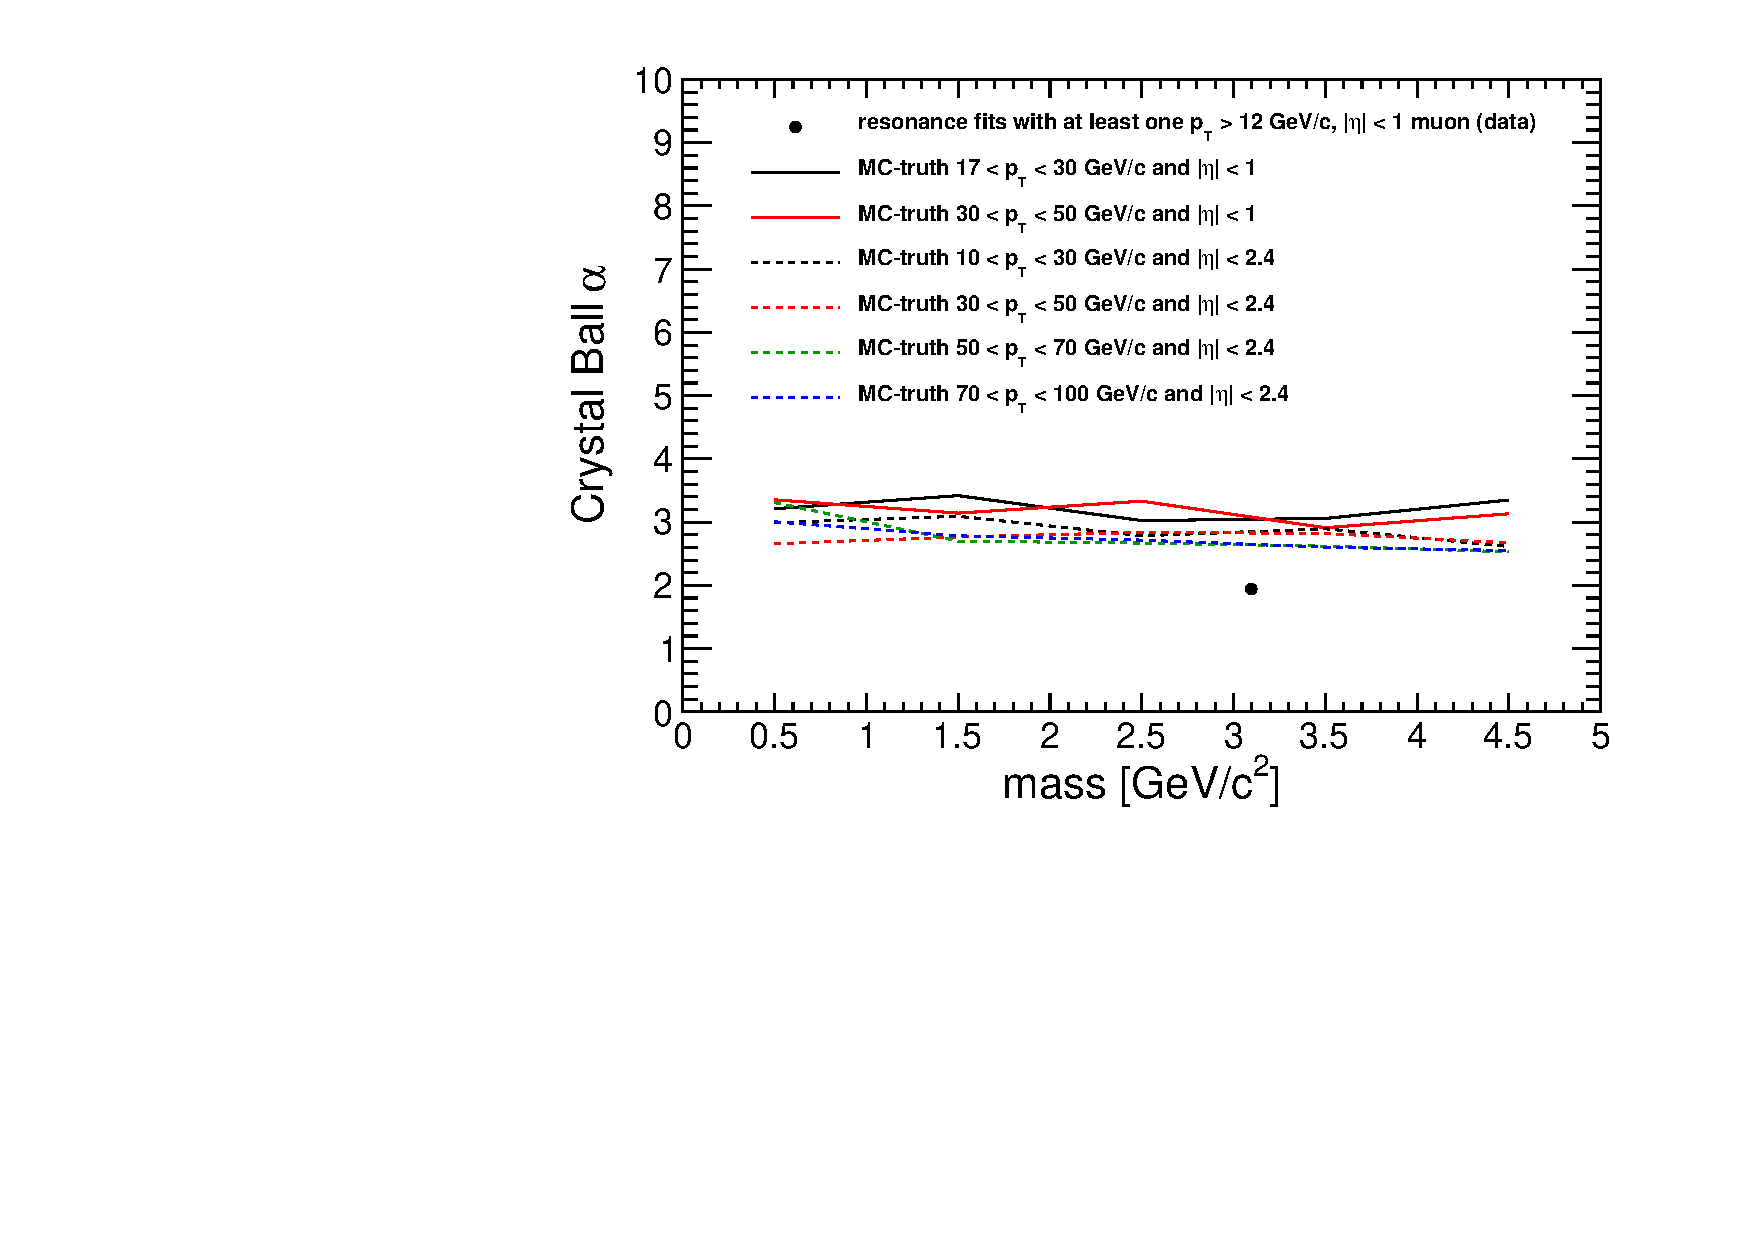
\includegraphics[width=0.5\linewidth]{resolution_alpha.pdf}
\end{frame}

\begin{frame}
\frametitle{Mass parameterization}
\framesubtitle{Crystal Ball function with $n=1$ (see Wikipedia)}

{\tt \tiny norm*((exp(-(x-mass)**2 / 2. / res**2) / sqrt(2.*3.1415926) / res)*((x-mass)/res > -alpha) + (0.4/res)*(exp(-alpha**2/2.)/abs(alpha)/(1./abs(alpha) - abs(alpha) - (x-mass)/res))*((x-mass)/res < -alpha))}

\begin{itemize}
\item {\tt norm} floats (cross-section limit parameter)
\item {\tt mass} is scanned from 0.3--5~GeV/$c^2$ (background
  parameteriztions are valid down to 0.3~GeV/$c^2$)
\item {\tt res} has two parameterizations:
\begin{itemize}
\item central: 0.007 + 0.006*mass {\scriptsize (nuisance parameter: allow the constant 0.007 to increase or decrease by at most 0.003)}

\item other: 0.007 + 0.010*mass {\scriptsize (same nuisance parameter)}

\end{itemize}
\item {\tt alpha} is somewhere between 2 and 3 {\scriptsize (another nuisance parameter)}
\end{itemize}

The ``central'' dimuon is either the only dimuon in the event (single dimuon channel) or is the dimuon that contains the most central muon with $p_T > 12$~GeV/$c$ (dimuon-dimuon channel)

{\scriptsize (When we require one $p_T > 12$~GeV/$c$, $|\eta| < 1$ muon in the event, the ``central'' dimuon is sufficient for triggering)}
\end{frame}

%% \section*{First section}
%% \begin{frame}
%% \begin{center}
%% \Huge \textcolor{blue}{First section}
%% \end{center}
%% \end{frame}

\begin{frame}
\frametitle{Issues and next steps}
\begin{itemize}
\item In the dimuon-dimuon channel, we can't simply randomize the two dimuons to make the plane symmetric.  Since we require one high-$p_T$ barrel muon to satisfy the trigger, we are effectively requiring one of the two dimuons to be higher-$p_T$ and in the barrel.  The other one is not constrained.  We therefore have an asymmetry we can't throw away: mass resolutions are different due to a looser $\eta$ requirement (pages 11, 12) and the shape of the backgrounds distribution is different due to a looser $p_T$ requirement (not shown here).  One axis will have to represent the ``central'' dimuon ($p_T > 17$~GeV/$c$, $|\eta| < 1$) while the other represents the ``other'' dimuon ($p_T > 10$~GeV/$c$, $|\eta| < 2.4$).  The mass template for the ``central'' dimuon is derived on page 6; to get a mass template for the ``other'' dimuon, we will need to use dimuon-muon events (3 muons total), where the trigger is satisfied by the ``orphan'' muon (we have enough data for the basic shape).
\item Mass templates for all channels with a quadmuon in it come from trimuon + track or dimuon + 2 tracks.  This is still on the to-do list.
\end{itemize}
\label{numpages}
\end{frame}

\end{document}
